\documentclass[12pt,a4paper]{report}
\usepackage[utf8]{vietnam}\usepackage{amsmath, amsthm, amssymb,latexsym,amscd,amsfonts,enumerate}
\usepackage[top=3.5cm, bottom=3.0cm, left=3cm, right=3.0cm]{geometry} 
\usepackage{color, fancyhdr, graphicx, wrapfig}
\usepackage[unicode]{hyperref}
\usepackage[vietnamese]{babel}
\usepackage{titling}
\usepackage{amsmath, amsthm, amssymb,latexsym,amscd,amsfonts,enumerate}
\usepackage{subfigure}
\usepackage{secdot}
\usepackage{graphicx}
\usepackage{booktabs}
\usepackage{amsthm}
\usepackage{amsmath}
\usepackage{amsfonts}
\usepackage{amssymb}
\usepackage{graphicx} 
\usepackage{titling}
\usepackage{secdot}
\usepackage{enumitem}
\usepackage{tikz}
\usepackage{array}
\usetikzlibrary{calc}
\usepackage{longtable}
\usepackage{indentfirst}
\usepackage{fancyhdr}
\usepackage{exscale,relsize,makeidx}
\usepackage{color, fancyhdr, graphicx, wrapfig}
\usepackage{amsmath}
\usepackage{textpos}
\usepackage{pgfplots}
\usepackage{tikz}
\usepackage{hyperref}
\usepackage{caption}
\usetikzlibrary{shapes.geometric, arrows}
\usetikzlibrary{datavisualization} 
\pgfplotsset{compat=1.18, width = 7cm}
\usetikzlibrary{patterns}
\usepackage{enumitem}
\usepackage{array}
\usepackage[tikz]{ocgx2}
\usepackage{xcolor}
\usepackage{blindtext}
\usepackage{multicol}
\usepackage{tikz}
\usepackage{subcaption}
\usepackage{changepage}
\usepackage{float}
\usepackage{pgfplotstable}
\usepackage{pgfplots}
\usepackage{blindtext}
\usepackage{titlesec}
\usepackage{mathtools}
\usepackage{tabularx}
\usepackage{nccmath}
\usetikzlibrary{calc}
\usepackage{longtable}
\usepackage{indentfirst}
\usepackage{fancyhdr}
\usepackage{exscale,relsize,makeidx}
%\usepackage{refcheck}
\setcounter{tocdepth}{4}
\setcounter{secnumdepth}{4}
\newtheorem{dn}{Định nghĩa}
\newtheorem{tc}{Tính chất}
\newtheorem{dl}{Định lý}
\newtheorem{md}{Mệnh đề}
\newtheorem{bd}{Bổ đề}
\newtheorem{hq}{Hệ quả}
\newtheorem{nx}{Nhận xét}
\newtheorem{vd}{Ví dụ}
\newtheorem{cm}{Chứng minh}
\newtheorem{cy}{Chú ý}
\newtheorem{ttoan}{Thuật toán}
\pagenumbering{roman}\pagestyle{plain}
%\pagestyle{fancy}
%\lhead{\it \changefontsizes{11pt}Luận văn thạc sĩ:}
%\rhead{\it Một số phương pháp vô hướng hóa cơ bản trong tối ưu đa mục tiêu}
%\lfoot{\it Nguyễn Văn Vân } 			         
%\rfoot{\it K19.2 trường ĐHSG}
\renewcommand{\headrulewidth}{1,2pt} 			
\renewcommand{\footrulewidth}{1,2pt}
\newcommand{\dstc}[2]
{
	\newdimen\stringwidth\setbox0=\hbox{#1}
	\stringwidth=\wd0
	\hspace*{-\parindent}\hspace*{.5\textwidth}\hspace*{-.5\wd0}#1\hfill #2\bigskip
	
}  
\usepackage{scrextend}
\fancyhf{}
\lhead{}
\chead{\thepage}
\rhead{}
\cfoot{}
\rfoot{}
\lfoot{}
\pagestyle{fancy}
\renewcommand{\headrulewidth}{1pt}
\begin{document} 
	\begin{titlepage}
		\begin{tikzpicture}[remember picture, overlay]
			\draw[line width = 1.5pt] ($(current page.north west) + (1in,-1in)$) rectangle ($(current page.south east) + (-0.6in,1in)$);
			
		\end{tikzpicture}
		\centering
		\textbf{ỦY BAN NHÂN DÂN THÀNH PHỐ HỒ CHÍ MINH\smallskip\\
			TRƯỜNG ĐẠI HỌC SÀI GÒN}\par
		\rule{5cm}{0.5pt}\par
		\vspace{2cm}
		{\Large\textbf{ĐỖ NGỌC MINH THƯ \\ NGUYỄN CHÍ BẰNG}\par}
		\vspace{4cm}
		{\Large\textbf{PHƯƠNG PHÁP GIẢI BÀI TOÁN\\ TỐI ƯU TUYẾN TÍNH NGUYÊN }\par}
		\vspace{4cm}
		\large\textbf{ ĐỀ TÀI NGHIÊN CỨU KHOA HỌC SINH VIÊN}\par		
		
		\large{CHUYÊN NGÀNH: TOÁN ỨNG DỤNG}
		\vspace{1.5cm}
		
		\vfill
		\textbf{Thành phố Hồ Chí Minh, năm 2024}
	\end{titlepage}
	\begin{titlingpage}
		\begin{tikzpicture}[remember picture, overlay]
			\draw[line width = 1.5pt] ($(current page.north west) + (1in,-1in)$) rectangle ($(current page.south east) + (-1in,1in)$);
			
		\end{tikzpicture}
		\centering
		\textbf{ỦY BAN NHÂN DÂN THÀNH PHỐ HỒ CHÍ MINH\smallskip\\
			TRƯỜNG ĐẠI HỌC SÀI GÒN}\par
		\rule{5cm}{0.5pt}\par
		\vspace{2cm}
		{\Large\textbf{ĐỖ NGỌC MINH THƯ \\ NGUYỄN CHÍ BẰNG}\par}
		\vspace{4cm}
		{\Large\textbf{PHƯƠNG PHÁP GIẢI BÀI TOÁN \\ TỐI ƯU TUYẾN TÍNH NGUYÊN}\par}
		\vspace{4cm}
		\large\textbf{ĐỀ TÀI NGHIÊN CỨU KHOA HỌC SINH VIÊN}\par		
		
		\large{CHUYÊN NGÀNH: TOÁN ỨNG DỤNG}
		\vspace{1.5cm}
		
		\large\textbf{Người hướng dẫn} \par
		\vspace{2cm}
		
		\large\textbf{PGS.TS. TẠ QUANG SƠN}\par
		
		%	\includegraphics[height=2cm]{chukynew}
		\vfill
		\textbf{Thành phố Hồ Chí Minh, năm 2024}
	\end{titlingpage}
	
	%\large
	\renewcommand{\baselinestretch}{1.2}
	\fontsize{13pt}{20pt}\selectfont
	
	\chapter*{Lời cam đoan}
	\thispagestyle{fancy}
	\addcontentsline{toc}{chapter}{Lời cam đoan}
	\vspace{1cm}
	\indent
	
	Chúng tôi tên là Đỗ Ngọc Minh Thư và Nguyễn Chí Bằng, là các  sinh viên lớp DTU1221, khoa Toán - Ứng dụng , khóa 2022-2026,  thuộc trường Đại học Sài Gòn. 
	
	Xin cam đoan rằng: Toàn bộ nội dung được trình bày trong đề tài  này này đều do chúng tôi thực hiện dưới sự hướng dẫn của PGS.TS. Tạ Quang Sơn.
	Những kết quả nghiên cứu của tác giả khác được sử dụng trong đề tài  đều có trích dẫn đầy đủ. 
	Chúng tôi xin chịu trách nhiệm nếu có các nội dung sao chép không hợp lệ hoặc vi phạm quy chế đào tạo. 
	\\
	\\
	\\
	\rightline{{\it {Tp. HCM, tháng ... năm 2024}} \hspace*{0cm}}
	\rightline{\textbf{Tác giả} \hspace*{2cm}}
	\\
	\\
	\\
	
	%\vspace*{1cm}
	\rightline{\textbf{Đỗ Ngọc Minh Thư}\hspace*{0.75cm}}
	
	\chapter*{Lời cảm ơn}
	\thispagestyle{fancy}
	\addcontentsline{toc}{chapter}{Lời cảm ơn}
	\vspace{1cm}
	\indent
	
	Đề tài nghiên cứu khoa học này được hoàn thành tại trường Đại Học Sài Gòn dưới sự hướng dẫn của PGS.TS. Tạ Quang Sơn.   Chúng em xin bày tỏ lòng biết ơn chân thành và sâu sắc về sự tận tâm và nhiệt tình của Thầy trong suốt quá trình thực hiện đề tài này.
	
	
	\bigskip
	Xin cám ơn Phòng Đào tạo  và Khoa Toán - Ứng dụng, Trường Đại học Sài Gòn, đã tạo nhiều điều kiện thuận lợi, giúp chúng em nâng cao chất lượng và nhiệm vụ học tập qua việc thực hiện đề tài này.
	\\
	\\
	\\
	\rightline{{\it {Tp. HCM, tháng ... năm 2024}} \hspace*{0cm}}
	\rightline{\textbf{Tác giả} \hspace*{2cm}}
	\\
	\\
	
	\vspace{1cm}
	\rightline{\textbf{Đỗ Ngọc Minh Thư} \hspace*{0.75cm}}
	\newpage
	
	\addcontentsline{toc}{chapter}{Mục lục}
	\tableofcontents
	%\thispagestyle{plain}
	\chapter*{Danh mục các kí hiệu}
	\thispagestyle{fancy}
	\addcontentsline{toc}{chapter}{Danh mục các kí hiệu}
	\begin{longtable}{l l}
		
		$\mathbb{R}$ & Tập các số thực\\
		%$\emptyset $ & Tập rỗng\\
		$\mathbb{R}^n$ & Không gian Euclide $n$-chiều\\

		
		$F$ & Tập chấp nhận được của bài toán tối ưu\\
		$\langle u, v \rangle$ & Tích vô hướng của hai véc tơ $u$ và $v$ trong $\mathbb{R}^n$\\
		
		
	\end{longtable}
\newpage
\pagenumbering{arabic} 
\chapter*{Lời nói đầu}
\thispagestyle{fancy}
\addcontentsline{toc}{chapter}{{\bf  Lời nói đầu}\rm}
\renewcommand{\baselinestretch}{1.2}
Thực tế cho thấy rằng trong nhiều bài toán tối ưu, nghiệm tìm được mong muốn phải là các số nguyên hoặc một bộ phận nghiệm của bài toán phải là các số nguyên. Điều này có thể thấy ở các bài toán như phân phối hàng hóa, sắp xếp tối ưu nhân lực, bài toán trên mạng, phân luồng giao thông,...
Đã từng có nhận định về việc tìm nghiệm nguyên của bài toán tối ưu là sau khi tìm được nghiệm tối ưu thì thưc hiện việc làm tròn nghiệm. Cách thức này thường không cho kết quả như mong muốn. Bởi lẽ nghiệm làm tròn có thể không thuộc miền chấp nhận được hoặc  có thể việc làm tròn như thế không chắc đã cho nghiệm tốt nhất như mong muốn. Lý thuyết về việc tìm nghiệm nguyên cho các bài toán tối ưu đáp ứng điều mong đợi nêu trên.

Bài toán tối ưu thường được xem xét dưới dạng 
$$
\begin{array}{ll}
{\rm Min\ (Max)}& f(x)\\
&x \in F,
\end{array}
$$
trong đó $f(x)$ là hàm mục tiêu tối ưu cần xác định, phụ thuộc vào biến $x$, xác định trên một không gian cho trước và $F$ là tập ràng buộc còn gọi là tập chấp nhận được. Mục tiêu của bài toán là đi tìm $x\in F$ sao cho hàm mục tiêu $f(x)$ đạt giá trị lớn nhất hay bé nhất.
Vì bài toán Max có thể đưa về bài toán Min và ngược lại, nên trong nhiều trường hợp để xây dựng các thuật toán tìm nghiệm cho bài toán, người ta chỉ cần xét một trong hai dạng nêu trên là đủ.



Trong đề tài này chúng tôi quan tâm tìm hiểu về nghiệm nguyên cho bài toán có hàm mục tiêu tuyến tính trên tập chấp nhận được xác định bởi các hàm tuyến tính. Bài toán có dạng như sau
$$
\begin{array}{ll}
{\rm Min}&\quad c_1x_1+\ldots+c_nx_n\\
{\rm s.t.}&\begin{cases}
a_{11}x_1+\ldots+a_{1n}x_n \le b_1\\
a_{21}x_1+\ldots+a_{2n}x_n \le b_2\\
\vdots\\
a_{m1}x_1+\ldots+a_{mn}x_n \le b_m\\
x_1, \ldots, x_n \ge 0.
\end{cases}
\end{array}
$$
Trong đó, $c_i, i=1,...,n$, các hệ số $a_{ij}$ với $i=1,...,m$ và $j=1,...,n$, và $b_i$ với $i=1,...,m$ là các số thực cho trước.

Bằng cách dùng ký hiệu véc tơ và ma trận, bài toán nêu trên được viết dưới dạng 
$$
\begin{array}{rl}
{\rm Min}& \langle c,x \rangle \\
{\rm s.t.}& 
\begin{cases}Ax \le b\\
 x\ge 0.
 \end{cases}
\end{array}
$$
Trong đó, cho trước $A$ là ma trận có $m$ dòng và $n$ cột, $c$ là véc tơ $n$ chiều và $b$ là véc tơ $m$ chiều. Chú ý rằng, các ràng buộc bất đẳng thức đều có thể biến đổi về ràng buộc đẳng thức. Vì thế trong nội dung của đề tài này, nếu không nói gì thêm, bài toán luôn được xét dưới dạng tổng quát
$$
\begin{array}{rl}
{\rm (IP) \; Min}& \langle c,x \rangle \\
{\rm s.t.}& 
\begin{cases}Ax = b\\
 x\ge 0.
 \end{cases}
\end{array}
$$

Các phương pháp mà đề tài này tìm hiểu là phương pháp sử dụng siêu phẳng cắt Gomory và phương pháp tìm nghiệm nguyên theo kiểu nhánh-cận do Land-Doig đề xuất. 

Nội dung đề tài được tổ chức thành 3 chương trong đó 

Chương 1; Dành để tóm lược lại một số kiến thức về Đại số tuyến tính liên quan đến véc tơ và ma trận. Đồng thời chương này cũng nhắc lại một số kết quả về phương pháp đơn hình khi giải bài toán quy hoạch tuyến tính.

Chương 2: Là phần chính của nội dung đề tài. Trong đó được chia làm hai phần. Phần đầu dành để trình bày phương pháp dùng siêu phẳng cắt Gomory và phần tiếp theo dành để trình bày phương pháp nhánh-cận kiểu Land-Doig. Trong mỗi phần đều có các ví dụ minh họa. Ngoài ra, dựa trên thực tế, khi sử dụng các phương pháp này để giải bài toán Quy hoạch nguyên, đề tài cũng đưa ra những nhận xét về phương pháp.

Phần cuối của đề tài này là Chương 3. Chúng tôi thử áp dụng các phương pháp trên để khảo sát việc tìm nghiệm nguyên cho bài toán dạng phân thức tuyến tính. 

Do lần đầu tham gia tập dượt nghiên cứu khoa học. Các tri thức chọn lọc và trình bày trong nội dung của đề tài này chưa đầy đủ hoặc còn sơ suất. Chúng em kính mong nhận được sự chỉ bảo từ quý thầy cô.

\newpage
\renewcommand{\baselinestretch}{1.2}
 
\chapter{Một số kiến thức cơ bản về bài toán quy hoạch tuyến tính} 
Kiến thức trình bày trong chương này, hầu hết được tham khảo từ các tài liệu  \cite{xxx} và \cite{xxx}.
\section{ Véc tơ, ma trận và các tính chất}

\subsection{ Véc tơ và các phép toán }
\begin{itemize}
\item Ký hiệu vector $x \in \mathbb{R}^n,$
\begin{equation*}
x=(x_1,x_2,\ldots,x_n).
\end{equation*}
Trong đó $x_i \in \mathbb{R}$ với $i=1,2,\ldots,n$.
\item Các phép toán:
\begin{equation*}
\begin{split}
x + y &= (x_1 + y_1, x_2 + y_2 , \ldots , x_n +y_n) \\
\lambda x &= (\lambda x_1 , \lambda x_2 , \ldots , \lambda x_n).
\end{split}
\end{equation*}
Trong đó $x, \: y \in \mathbb{R}^n$ và $\lambda \in \mathbb{R}$.
\item Thứ tự vector: 
\begin{equation*}
\begin{split}
x \leq y & \Leftrightarrow x_i \leq y_i, \\
x < y & \Leftrightarrow x_i < y_i, \\
x = y & \Leftrightarrow x_i = y_i. \\
\end{split}
\end{equation*}
Trong đó $i=1,2,\ldots,n$.
\item Vector đơn vị: $(1,0,\ldots,0),\:(0,1,\ldots,0) , \ldots , (0,0,\ldots,1)$.
\item Vector $0$: $0=(0,0,\ldots,0)$. 
\end{itemize}

\subsection{ Ma trận và các phép toán}
\begin{itemize}
\item Ký hiệu $A$ là ma trận $m\times n$, trong đó $A=(a_{ij})$ và $i=1,2,\ldots,m$, $j=1,2,\ldots,n$. $A_i$ chỉ dòng thứ $i$ của ma trận $A$ và $A_j$ chỉ cột thứ $j$ của ma trận $A$.
\item $A$ là ma trận vuông khi $m=n$.
\item Ma trận cột:
\begin{equation*}
A = \begin{bmatrix}
        a_1 \\
        a_2 \\
        \vdots \\
        a_n
	\end{bmatrix}.
\end{equation*}
\item Ma trận dòng:
\begin{equation*}
A^T = \begin{bmatrix}
	a_1 & a_2 & \cdots & a_n
	\end{bmatrix}.
\end{equation*}
\item Ma trận đơn vị:
\begin{equation*}
I = \begin{bmatrix}
        1 & 0 & \cdots & 0 \\
		0 & 1 & \cdots & 0 \\
		\vdots & \vdots & \ddots & \vdots \\
		0 & 0 & \cdots & 1
	\end{bmatrix}.
\end{equation*}
\item Cộng ma trận: $A, \: B$ là ma trận $m\times n$,
\begin{equation*}
A + B = (a_{ij}+b_{ij}).
\end{equation*}
Trong đó $i=1,2,\ldots,m$ và $j=1,2,\ldots,n$.
\item Nhân với 1 số: $A, \: B$ là ma trận $m\times n$,
\begin{equation*}
\lambda A = (\lambda a_{ij}).
\end{equation*}
Trong đó $i=1,2,\ldots,m$ và $j=1,2,\ldots,n$.
\item Với ma trận dòng
\begin{equation*}
A^T = \begin{bmatrix}
	a_1 & a_2 & \cdots & a_n
	\end{bmatrix}.
\end{equation*}
và ma trận cột
\begin{equation*}
B = \begin{bmatrix}
        b_1 \\
        b_2 \\
        \vdots \\
        b_n
	\end{bmatrix}.
\end{equation*}
Ta có tích hai ma trận
\begin{equation*}
A\times B = a_1b_1 + a_2b_2 + \ldots + a_nb_n.
\end{equation*}
\item Tích của ma trận $A$ cấp $m \times p$ với ma trận $B$ cấp $p \times n$ ta được ma trận $C$ cấp $m \times n$:
\begin{equation*}
C = \begin{bmatrix}
        A_1B^1 & A_1B^2 & \cdots & A_1B^n  \\
		A_2B^1 & A_2B^2 & \cdots & A_2B^n \\
		\vdots & \vdots & \ddots & \vdots \\
		A_mB^1 & A_mB^2 & \cdots & A_mB^n
	\end{bmatrix}.
\end{equation*}
\item Hệ phương trình
\begin{equation*}
\left\{\begin{split}
\begin{matrix}
& a_{11}x_1 & + & a_{12}x_2 & + & \cdots & + & a_{1n}x_n & = & b_1 \\
& a_{21}x_1 & + & a_{22}x_2 & + & \cdots & + & a_{2n}x_n & = & b_2 \\
&&&&& \vdots \\
& a_{m1}x_1 & + & a_{m2}x_2 & + & \cdots & + & a_{mn}x_n & = & b_m \\
\end{matrix},
\end{split}\right.  
\end{equation*}
có thể viết lại thành
\begin{equation}
\begin{bmatrix}
	a_{11} & a_{12} & \cdots & a_{1n} \\
	a_{21} & a_{22} & \cdots & a_{2n} \\
	\vdots & \vdots & \ddots & \vdots \\
	a_{m1} & a_{m2} & \cdots & a_{mn} 
\end{bmatrix}
\begin{bmatrix}
	x_1 \\
	x_2 \\
	\vdots \\
	x_m
\end{bmatrix}
=
\begin{bmatrix}
	b_1 \\
	b_2 \\
	\vdots \\
	b_m
\end{bmatrix}.
\end{equation}

\end{itemize}

\subsection{Các phép biến đổi trên ma trận}
\begin{itemize}
\item Các phép biến đổi bao gồm:
\begin{itemize}
\item \textbf{Phép đổi hàng.} Đổi chỗ hàng $i$ và hàng $j$ của ma trận, được ký hiệu $h_i \leftrightarrow h_j$.
\item \textbf{Phép thay thế tỷ lệ.} Nhân hàng $i$ của ma trận với số $\alpha \neq 0$, được ký hiệu $h_i \leftarrow \alpha h_i$.
\item \textbf{Phép thay thế hàng.} Cộng vào hàng $i$ một bội $k$ lần hàng $j$, được ký hiệu là $h_i \leftarrow h_i + k h_j$, với $j \neq i$.
\end{itemize}
\end{itemize}

\subsection{ Định thức của ma trận và ma trận đảo}
Cho ma trận vuông cấp $n$:
\begin{equation*}
A =
\begin{bmatrix}
	a_{11} & a_{12} & \cdots & a_{1n} \\
	a_{21} & a_{22} & \cdots & a_{2n} \\
	\vdots & \vdots & \ddots & \vdots \\
	a_{n1} & a_{n2} & \cdots & a_{nn} 
\end{bmatrix}
\end{equation*}
\begin{itemize}
\item Định thức của ma trận $A$ được tính theo công thức:
\begin{equation}
\text{det}(A) = \sum _{\sigma \in S_n} \text{sgn} (\sigma) \prod _{i=1}^n a_{i,\sigma (i)}.
\end{equation}
\item Ta có thể viết định thức của ma trận $A$ dưới dạng
\begin{equation*}
\text{det} A =
\begin{vmatrix}
	a_{11} & a_{12} & \cdots & a_{1n} \\
	a_{21} & a_{22} & \cdots & a_{2n} \\
	\vdots & \vdots & \ddots & \vdots \\
	a_{n1} & a_{n2} & \cdots & a_{nn} 
\end{vmatrix}.
\end{equation*}
\item Áp dụng vào ma trận vuông cấp 1, ta có:
\begin{equation}
\text{det}[a]=a.
\end{equation}
\item Áp dụng vào ma trận vuông cấp 2, ta có:
\begin{equation}
\text{det} \begin{bmatrix}
a_{11} & a_{12} \\
a_{21} & a_{22}
\end{bmatrix} = \begin{vmatrix}
a_{11} & a_{12} \\
a_{21} & a_{22}
\end{vmatrix} = a_{11}a_{22} - a_{12}a_{21}.
\end{equation}
\end{itemize}
Ma trận vuông $B$ được gọi là ma trận đảo của $A$ nếu $AB=BA=I$.

\textbf{Ví dụ.} Cho hai ma trận
\begin{equation*}
A = \begin{pmatrix}
	1 & -2 \\
	1 & -1
	\end{pmatrix}
\text{ và }
B = \begin{pmatrix}
	-1 & 2 \\
	-1 & 1
	\end{pmatrix},
\end{equation*}
\hspace*{2cm} ta có $AB=BA=I$.
\section{Một số kiến thức cơ bản về Bài toán tối ưu tuyến tính}

\subsection{Bài toán dạng chính tắc và chuẩn tắc}
\begin{itemize}
    \item \textbf{Bài toán dạng chính tắc}
    
    Ta có bài toán dạng:
    \begin{equation} \small \label{F}
        \begin{split}
        f(x) & = c^Tx \quad \longrightarrow \text{Min} \\
            & \left\{
            \begin{split}
            & \sum _{j=1}^n a_{ij} x_j = b_i, \: i=1,2,\ldots,m \\
            & x_j \geq 0, \: j=1,2,\ldots,n.
            \end{split}
            \right.    
        \end{split}
    \end{equation}

    Thì ta gọi bài toán trên có dạng chính tắc và có thể viết lại dưới dạng:

    \begin{equation} \small \label{chinhtac}
        \begin{split}
        (P) \quad \text{Min } & f(x) = c^Tx \\
            & \left\{
            \begin{split}
            & Ax=b, \\
            & x_j \geq 0.
            \end{split}
            \right.    
        \end{split}
    \end{equation}

    Trong đó $A$ là ma trận $m\times n$, $b=\begin{pmatrix}
        b_1 \\
        b_2 \\
        \vdots \\
        b_m
        \end{pmatrix}$ và $c^T=(c_1 \: c_2 \: \ldots \: c_n)$.

    \item \textbf{Bài toán dạng chuẩn tắc}
    
    Nếu bài toán có dạng:

    \begin{equation} \small \label{F}
        \begin{split}
        f(x) & = c^Tx \quad \longrightarrow \text{Min} \\
            & \left\{
            \begin{split}
            & \sum _{j=1}^n a_{ij} x_j \geq b_i, \: i=1,2,\ldots,m \\
            & x_j \geq 0, \: j=1,2,\ldots,n.
            \end{split}
            \right.    
        \end{split}
    \end{equation}

    Thì ta gọi bài toán trên có dạng chuẩn tắc và có thể viết lại dưới dạng:

    \begin{equation} \small \label{F}
        \begin{split}
        (P) \quad \text{Min } & f(x) = c^Tx \\
            & \left\{
            \begin{split}
            & Ax \geq b, \\
            & x_j \geq 0.
            \end{split}
            \right.    
        \end{split}
    \end{equation}

    Tương tự $A$ là ma trận $m\times n$, $b=\begin{pmatrix}
        b_1 \\
        b_2 \\
        \vdots \\
        b_m
        \end{pmatrix}$ và $c^T=(c_1 \: c_2 \: \ldots \: c_n)$.

\end{itemize}

\subsection{Chuyển bài toán về dạng chính tắc}

Để thuận tiện, ta chỉ xét dạng bài toán quy hoạch tuyến tính tổng quát là \textbf{dạng chính tắc} và bất kỳ bài toán nào cũng có thể đưa về dạng chính tắc.

\begin{itemize}
\item \textbf{Phương pháp đưa về dạng chính tắc:}
    \begin{itemize}
    \item Bài toán $\max f(x) \longrightarrow -\min [-f(x)]$.
    \item Bằng cách thêm ẩn phụ $x_{n+i}$ tương ứng có hệ số trong hàm mục tiêu là $c_{n+i}=0$, ta có thể đưa bất đẳng thức 
    \begin{equation*}
    \sum _{j=1}^n a_{ij} x_j \geq b_i
    \end{equation*}
    hoặc
    \begin{equation*}
    \sum _{j=1}^n a_{ij} x_j \leq b_i
    \end{equation*}
    lần lượt thành đẳng thức
    \begin{equation*}
    \sum _{j=1}^n a_{ij} x_j - x_{n+i} = b_i
    \end{equation*}
    hoặc
    \begin{equation*}
    \sum _{j=1}^n a_{ij} x_j + x_{n+i} = b_i
    \end{equation*}
    \item Nếu tồn tại bất kỳ $x_k$ không có ràng buộc thì ta viết
    \begin{equation*}
    x_k = x_k^{'} - x_k^{''}
    \end{equation*}
    với $x_k^{'} \geq 0$ và $x_k^{''} \geq 0$.
    \end{itemize}
\end{itemize}
Kể từ đây, ta chỉ quan tâm bài toán \eqref{chinhtac}.


\section{Phương pháp giải bài toán tối ưu tuyến tính}

\subsection{Phương pháp hình học}
\subsubsection*{Vấn đề về tập lồi}
\usetikzlibrary{patterns}

\begin{dn}[Tập lồi]
Tập $S$ được gọi là \textbf{tập lồi} nếu $S$ thoả điều kiện:
\begin{itemize}
\item Cho bất kỳ 2 điểm $A$ và $B$ nằm trong tập $S$.
\item Đường thẳng nối 2 điểm $A$ và $B$ luôn nằm trong $S$.
\end{itemize}
\end{dn}


\begin{dn}[Cực điểm]
Với bất kỳ tập $S$, điểm $P \in S$ được gọi là \textbf{cực điểm} nếu thoả các điều kiện:
\begin{itemize}
\item Tồn tại đoạn thẳng $AB$ nằm hoàn toàn trong $S$.
\item Tồn tại điểm $P$ sao cho $P := \{x \in AB: x=A \vee x=B \}$.
\end{itemize}
\end{dn}

\begin{dn}[Siêu phẳng]
Tập $S$ gọi là một \textbf{siêu phẳng} nếu $S$ gồm các vector
\begin{equation*}
X = \begin{bmatrix}
        x_1 \\
        x_2 \\
        \vdots \\
        x_n
	\end{bmatrix}
\end{equation*}
trong không gian $\mathbb{R}^n$ sao cho
\begin{equation*}
a_1x_1 + a_2x_2 + \ldots + a_nx_n = c
\end{equation*}
trong đó $c$ là một hằng số và $a_1,a_2,\ldots,a_n \neq 0$.
\end{dn}
\begin{figure}
	\centering
	\subfigure[]{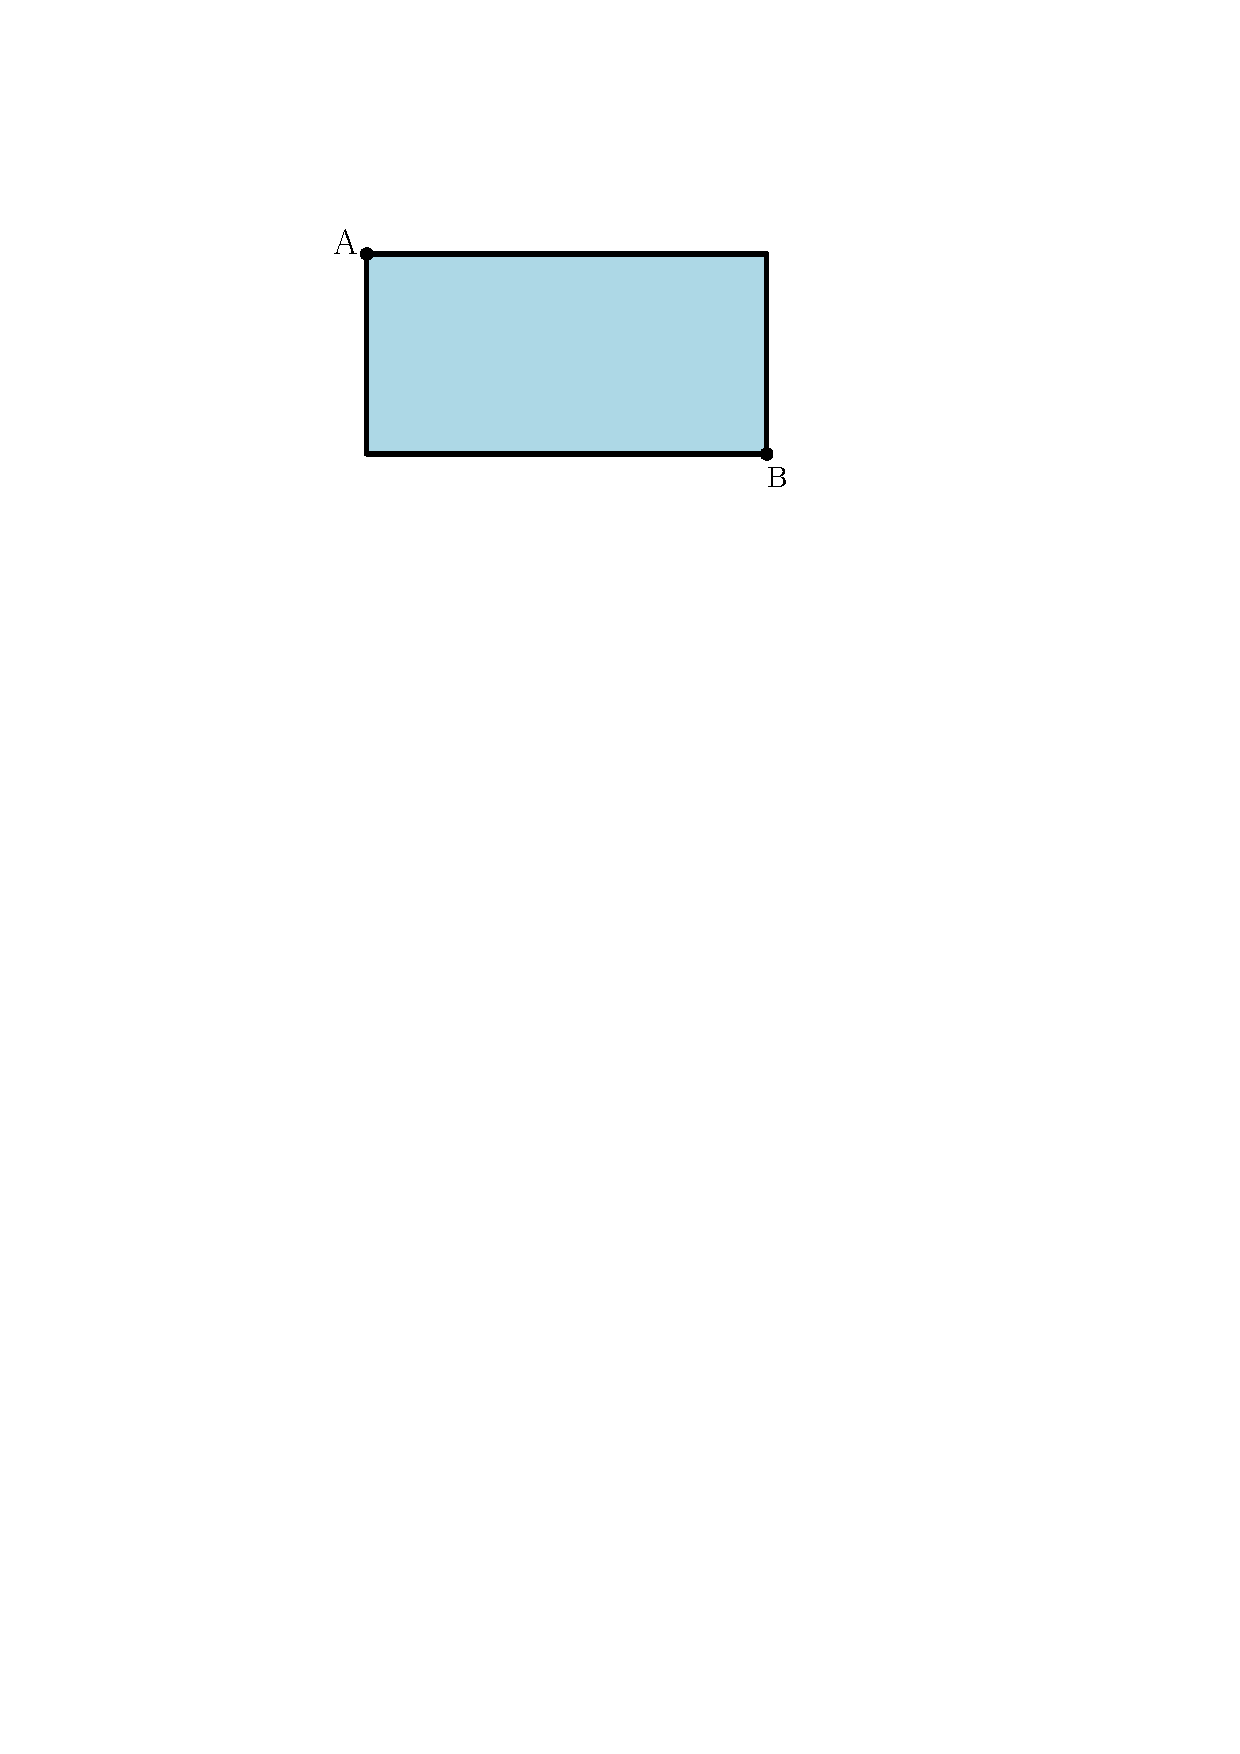
\includegraphics[width=0.2\textwidth]{vuong2.pdf}} 
	\subfigure[]{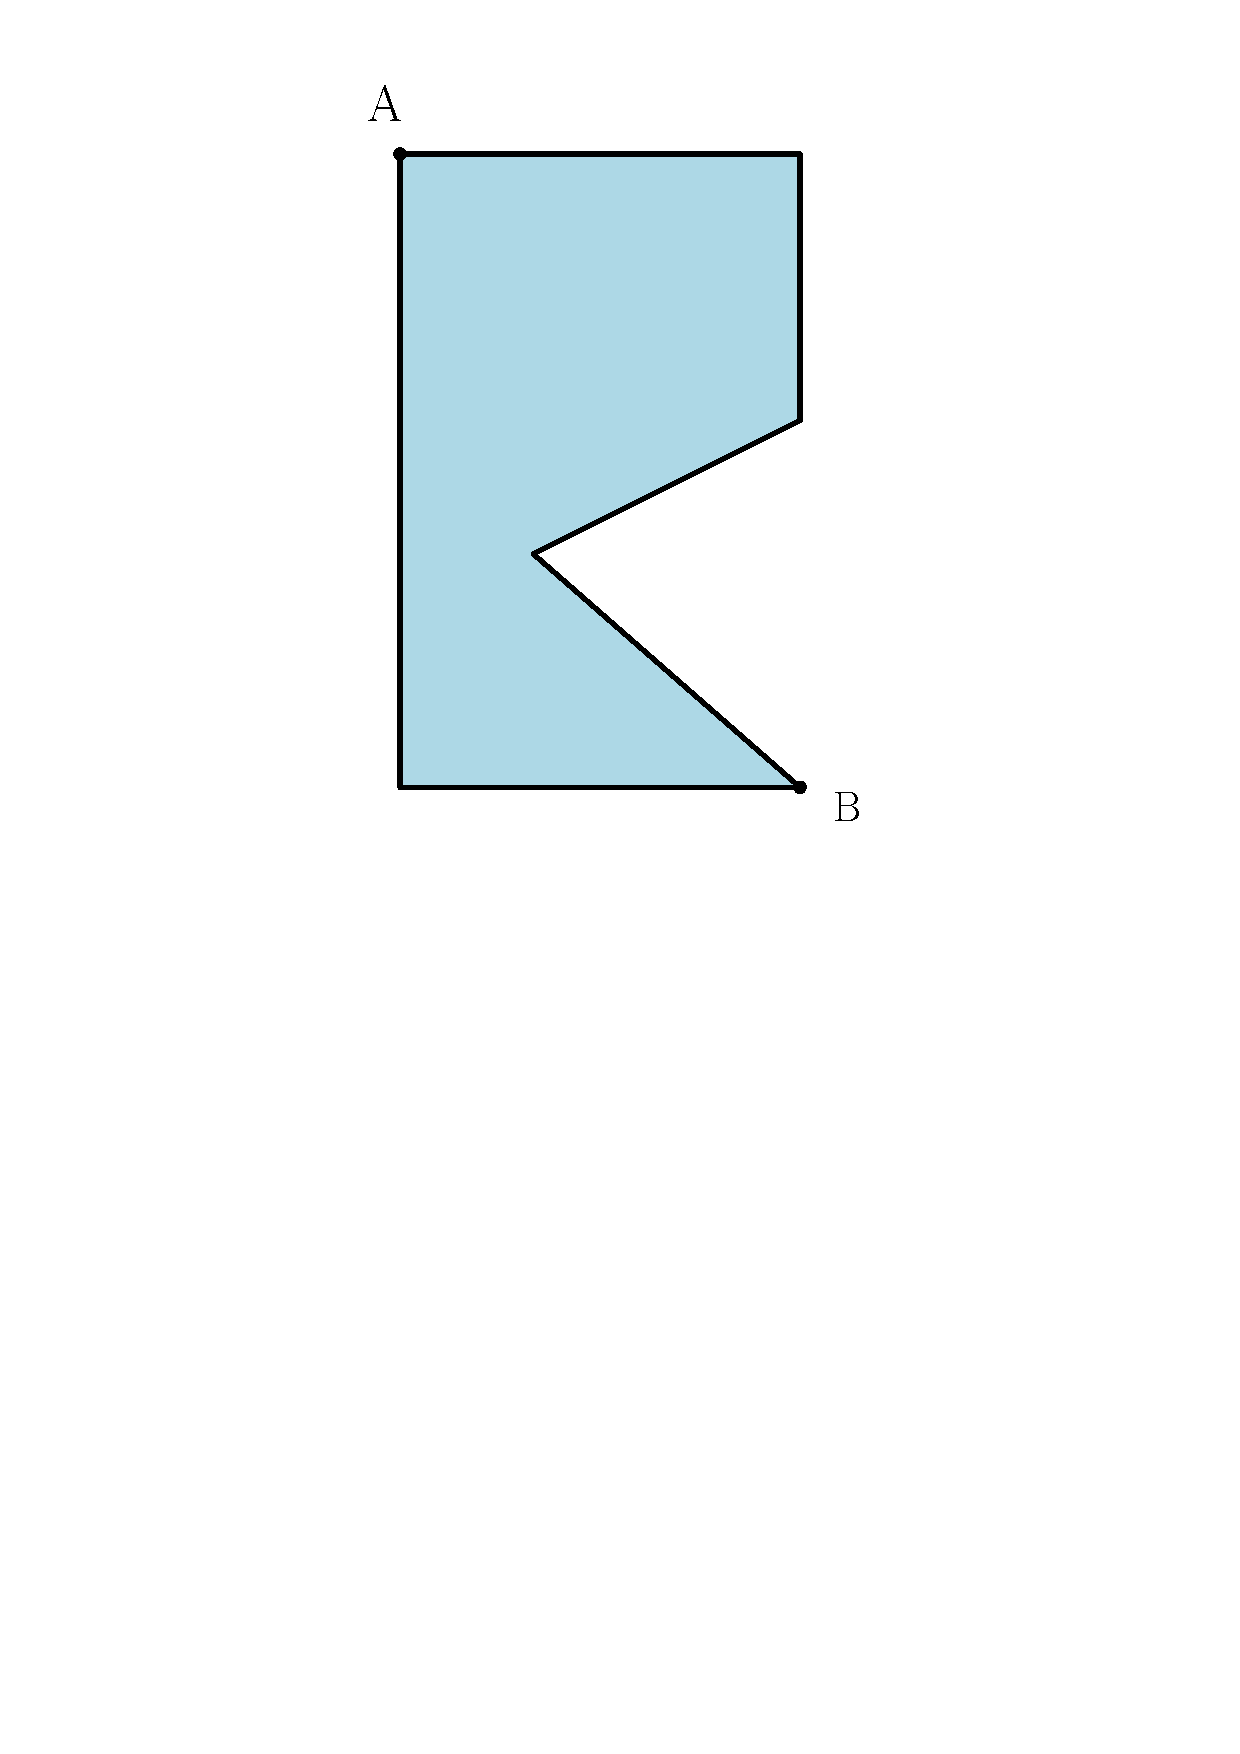
\includegraphics[width=0.15\textwidth]{lom.pdf}} 
	\subfigure[]{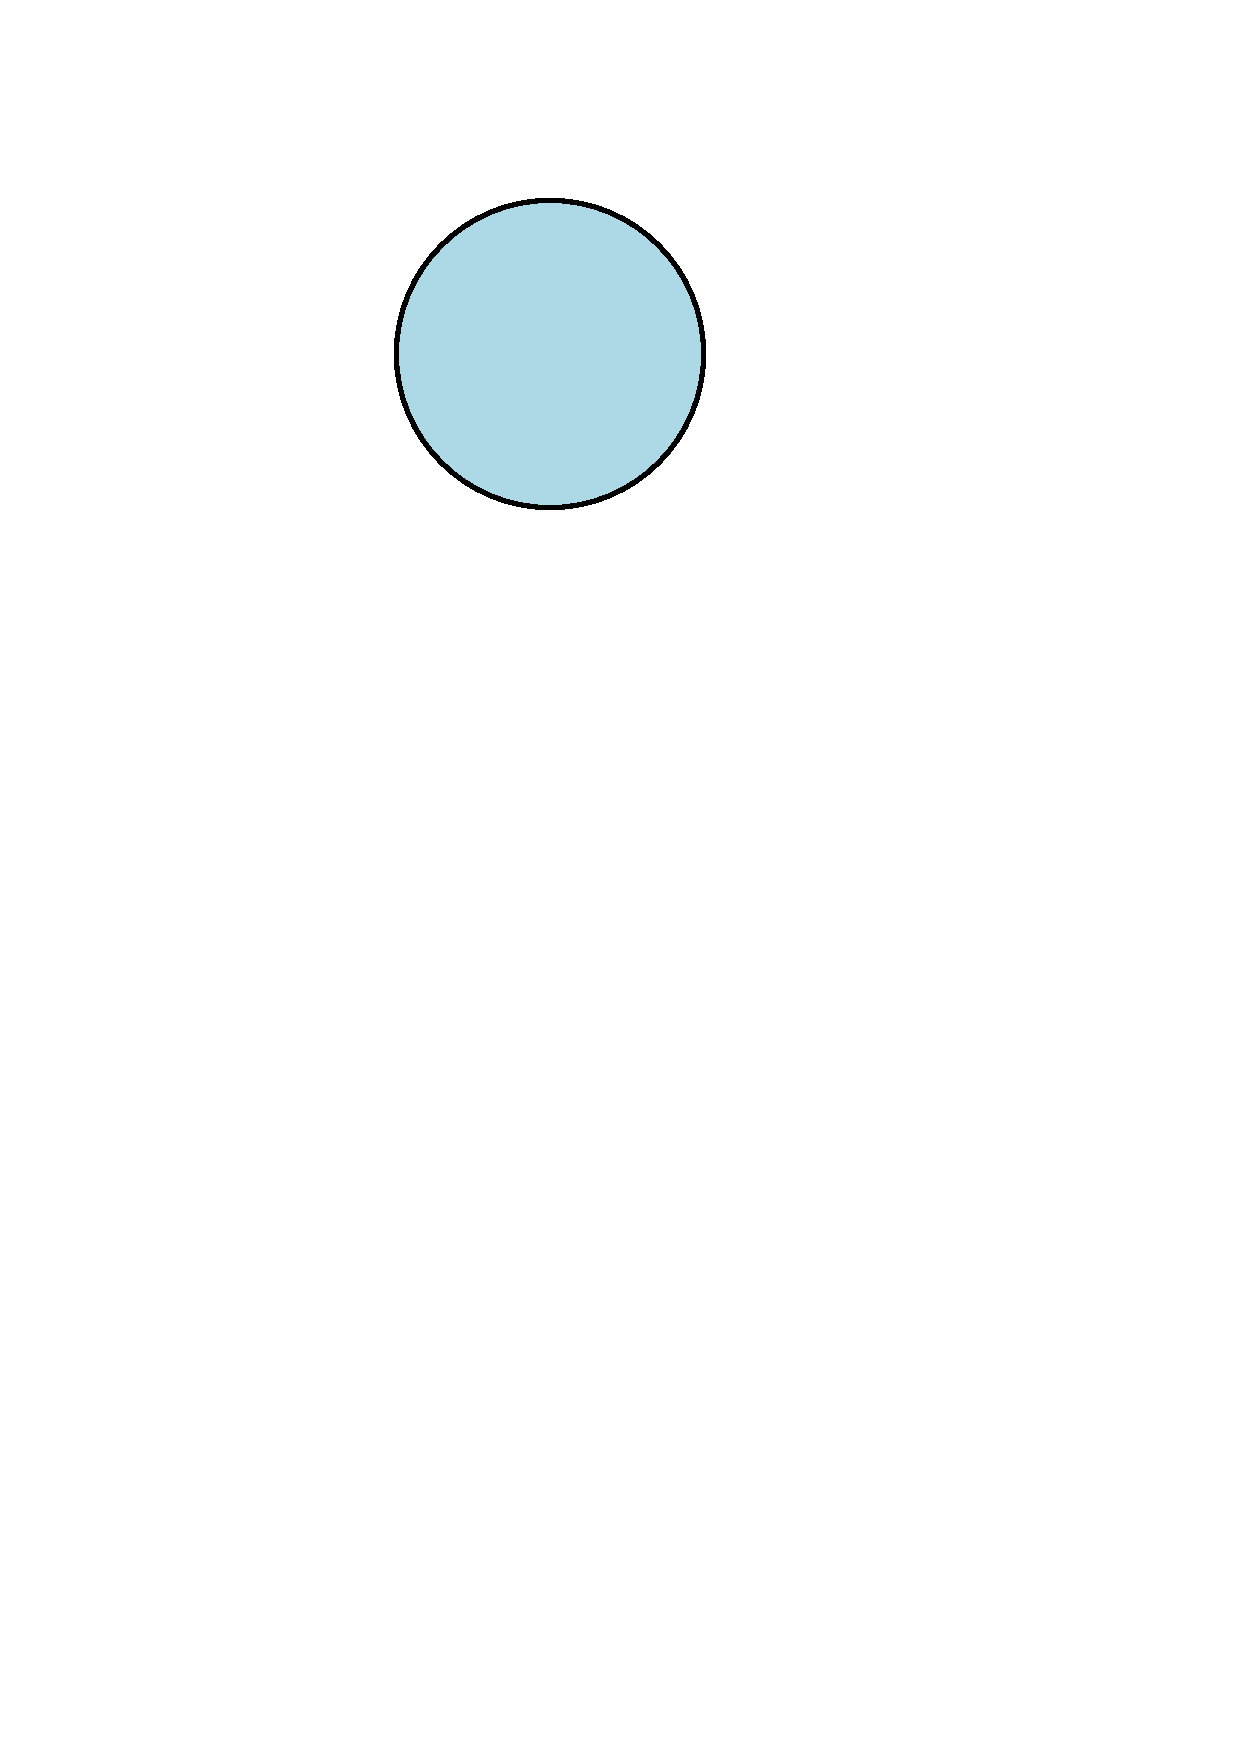
\includegraphics[width=0.15\textwidth]{tron.pdf}} 
	\subfigure[]{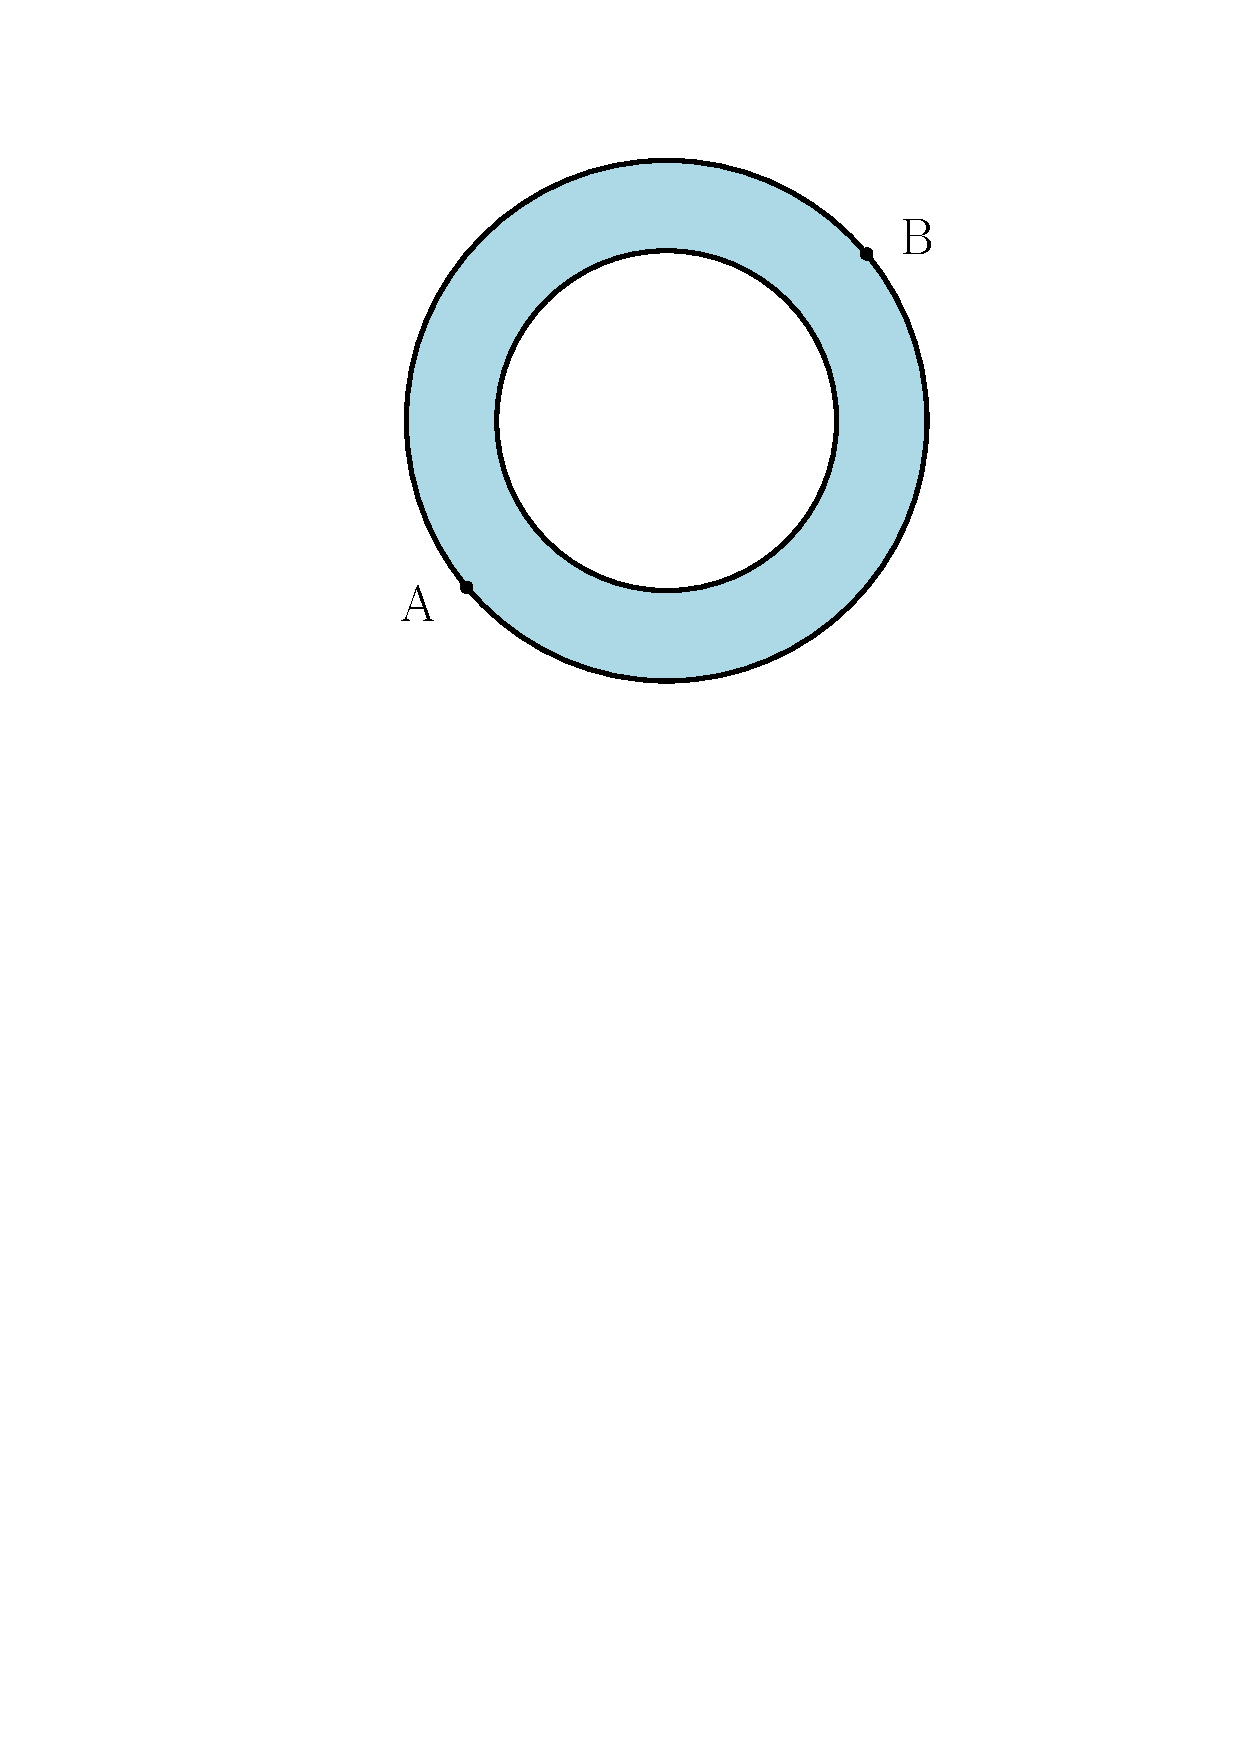
\includegraphics[width=0.15\textwidth]{duc lo.pdf}} 
	\caption{(a) Tập lồi (b) Tập lõm (c) Tập lồi (d) Tập lõm}
	\label{fig:foobar}
\end{figure}

\subsubsection*{Bài toán trong không gian $\mathbb{R}^2$}

\begin{equation} \small \label{chinhtac}
	\begin{split}
	(P) \quad \text{Min } & f(x) = c^Tx \\
		& \left\{
		\begin{split}
		& Ax=b, \\
		& x_j \geq 0, \:\: j=1,2.
		\end{split}
		\right.    
	\end{split}
\end{equation}
Trong đó $A$ là ma trận $m\times 2$, $b=\begin{pmatrix}
	b_1 \\
	b_2 \\
	\vdots \\
	b_m
	\end{pmatrix}$ và $c^T=(c_1 \: c_2 )$.


\begin{itemize}
\item \textbf{Tập nghiệm của bài toán}

Ta có bài toán minh hoạ sau:
\begin{equation}
	\begin{split}
	(P) \quad & f(x) = 3x_1 + 2x_2 \longrightarrow Max \\
		& \left\{\begin{split}
		x_1 + x_2 &\leq 7 \\
		2x_1 + x_2 &\leq 10 \\
		x_1 &\leq 4 \\
		x_1, x_2 &\geq 0. \\
		\end{split}\right.    
	\end{split}
\end{equation}
Với từng ràng buộc, ta có thể biểu thị trên đồ thị bằng từng đường thẳng tương ứng, ví dụ, ràng buộc
\begin{equation*}
x_1 + x_2 \leq 7
\end{equation*}
tương ứng với mặt phẳng bên dưới đường thẳng $CD$ trong hình 2.
\begin{equation*}
	2x_1 + x_2 \leq 10
\end{equation*}
tương ứng với mặt phẳng bên dưới đường thẳng $AB$.
\begin{equation*}
	x_1 \leq 4
	\end{equation*}
tương ứng với mặt phẳng bên trái đường thẳng $EG$. Tập nghiệm của bài toán là đa giác $OCKGE$ được biểu thị trong đồ thị hình 2.

\item \textbf{Phương án tối ưu của bài toán}
\begin{itemize}
\item Để tìm phương án tối ưu của bài toán ta thiết lập phương thay đổi của hàm mục tiêu
\begin{equation*}
f(x)=c_1x_1+c_2x_2,
\end{equation*}
trong đó phương trình mô tả họ đường thẳng phụ thuộc theo tham số $f(x)$ với pháp vector $v=(c_1,c_2)$, giá trị $f(x)$ tăng hoặc giảm theo một hướng của vector v.
\item Từ phương trình hàm mục tiêu ta thiết lập các đường mức.
\item Tịnh tiến song song các đường mức theo chiều tăng nếu Max hoặc giảm nếu Min để tìm phương án tối ưu của bài toán. (Hình 3)
\end{itemize}

\begin{figure}[!htb]\label{hinh2}
    \begin{minipage}{0.48\textwidth}
            \center
            \begin{tikzpicture}
            \begin{axis}
                [
                xmin=0,xmax=10,
                ymin=0,ymax=15,
                xlabel={$x_1$},
                ylabel={$x_2$},
                grid style={line width=.1pt, draw=darkgray!50},
                major grid style={line width=.2pt,draw=darkgray!50},
                axis lines=middle,
                yticklabel=\empty,
                xticklabel=\empty,
                enlargelimits={abs=0},
                samples=10,
                domain = 0:1,
                ]
                \filldraw[blue!50, pattern=north west lines, pattern color=blue!90, line width=1.5pt] (0, 0) -- (0, 7) -- (3, 4) -- (4, 2) -- (4, 0) -- cycle;
                \draw (0, 7) -- (7, 0);
                \draw (0, 10) -- (5, 0);
                \draw (4, 0) -- (4, 9);
                \node at (0.3, 0.4) {\tiny O};
                \node at (0.4, 7.2) {\tiny C};
                \node at (4.2, 0.4) {\tiny E};
                \node at (4.3, 2) {\tiny G};
                \node at (3.2, 4.3) {\tiny K};
                \node at (7.2, 0.4) {\tiny D};
                \node at (5.2, 0.4) {\tiny B};
                \node at (0.5, 10) {\tiny A};
                \node at (0, 7) {\tiny \textbullet};
                \node at (3, 4) {\tiny \textbullet};
                \node at (4, 2) {\tiny \textbullet};
                \node at (4, 0) {\tiny \textbullet};
                \node at (5, 0) {\tiny \textbullet};
                \node at (7, 0) {\tiny \textbullet};
            \end{axis}
            \end{tikzpicture}  
            \caption{Đa giác $OCKGE$ là tập nghiệm của bài toán (P).}
    \end{minipage}\hfill
    \begin{minipage}{0.48\textwidth}
            \center
            \begin{tikzpicture}
            \begin{axis}
                [
                xmin=0,xmax=10,
                ymin=0,ymax=15,
                xlabel={$x_1$},
                ylabel={$x_2$},
                grid style={line width=.1pt, draw=darkgray!50},
                major grid style={line width=.2pt,draw=darkgray!50},
                axis lines=middle,
                yticklabel=\empty,
                xticklabel=\empty,
                enlargelimits={abs=0},
                samples=10,
                domain = 0:1,
                ]
                \filldraw[blue!30, pattern=north west lines, pattern color=blue!30, line width=1pt] (0, 0) -- (0, 7) -- (3, 4) -- (4, 2) -- (4, 0) -- cycle;
                \draw (0, 7) -- (7, 0);
                \draw (0, 10) -- (5, 0);
                \draw (4, 0) -- (4, 9);
                \draw[dotted, line width = 1.5pt] (0, 8) -- (6, 0);
                \draw[->, line width = 1.5pt] (0, 0) -- (1.5, 2);
                \node at (0.4, 7.2) {\tiny C};
                \node at (4.2, 0.4) {\tiny E};
                \node at (4.3, 2) {\tiny G};
                \node at (3.4, 4.5) {\small \textbf{K}};
                \node at (7.2, 0.4) {\tiny D};
                \node at (5.2, 0.4) {\tiny B};
                \node at (0.5, 10) {\tiny A};
                \node at (0, 10) {\tiny \textbullet};
                \node at (0, 7) {\tiny \textbullet};
                \node at (3, 4) {\small \textbullet};
                \node at (4, 2) {\tiny \textbullet};
                \node at (4, 0) {\tiny \textbullet};
                \node at (5, 0) {\tiny \textbullet};
                \node at (7, 0) {\tiny \textbullet};
            \end{axis}
            \end{tikzpicture}  
            \caption{Minh hoạ phương pháp tìm phương án tối ưu của bài toán (P).}
    \end{minipage}
 \end{figure}

\end{itemize}

\subsection*{Các trường hợp đặc biệt}
\textbf{Trường hợp bài toán vô nghiệm}

Trường hợp bài toán có các ràng buộc không cùng tạo ra miền nghiệm của bài toán, xem Hình 4. thì bài toán được gọi là vô nghiệm.

\textbf{Trường hợp bài toán vô số nghiệm}

Trường hợp bài toán có đường mức được tạo ra từ phương trình hàm mục tiêu song song với cực biên của tập nghiệm, bài toán cho ra vô số nghiệm. (Hình 5)
\begin{figure}[!htb]
    \begin{minipage}{0.48\textwidth}
    \center
    \begin{tikzpicture}
    \begin{axis}
        [
        xmin=0,xmax=10,
        ymin=0,ymax=15,
        xlabel={$x_1$},
        ylabel={$x_2$},
        grid style={line width=.1pt, draw=darkgray!50},
        major grid style={line width=.2pt,draw=darkgray!50},
        axis lines=middle,
        yticklabel=\empty,
        xticklabel=\empty,
        enlargelimits={abs=0},
        samples=10,
        domain = 0:1,
        ]
        \draw (0, 7) -- (7, 0);
        \draw (0, 10) -- (5, 0);
        \draw (6, 0) -- (6, 9);
        \draw (0, 4) -- (8, 4);
        \node at (0.3, 0.4) {\tiny O};
        \node at (0.4, 7.2) {\tiny C};
        \node at (3.2, 4.5) {\tiny K};
        \node at (7.2, 0.4) {\tiny D};
        \node at (5.2, 0.4) {\tiny B};
        \node at (0.5, 10) {\tiny A};
        \node at (0, 10) {\tiny \textbullet};
        \node at (0, 7) {\tiny \textbullet};
        \node at (3, 4) {\tiny \textbullet};
        \node at (5, 0) {\tiny \textbullet};
        \node at (7, 0) {\tiny \textbullet};
        \node at (0, 0) {\tiny \textbullet};
    \end{axis}
    \end{tikzpicture}  
    \caption{Minh hoạ trường hợp bài toán vô nghiệm.}
    \end{minipage}\hfill
    \begin{minipage}{0.48\textwidth}
    \center
    \begin{tikzpicture}
    \begin{axis}
        [
        xmin=0,xmax=10,
        ymin=0,ymax=15,
        xlabel={$x_1$},
        ylabel={$x_2$},
        grid style={line width=.1pt, draw=darkgray!50},
        major grid style={line width=.2pt,draw=darkgray!50},
        axis lines=middle,
        yticklabel=\empty,
        xticklabel=\empty,
        enlargelimits={abs=0},
        samples=10,
        domain = 0:1,
        ]
        \filldraw[blue!30, pattern=north west lines, pattern color=blue!30, line width=1pt] (0, 0) -- (0, 7) -- (3, 4) -- (4, 2) -- (4, 0) -- cycle;
        \draw (0, 7) -- (7, 0);
        \draw (0, 10) -- (5, 0);
        \draw (4, 0) -- (4, 9);
        \draw[dotted, line width=2pt] (0, 2.594) -- (1.3, 0);
        \draw[->] (0, 0) -- (2, 3);
        \node at (0.4, 7.2) {\tiny C};
        \node at (4.2, 0.4) {\tiny E};
        \node at (4.3, 2) {\tiny G};
        \node at (3.2, 4.3) {\tiny K};
        \node at (7.2, 0.4) {\tiny D};
        \node at (5.2, 0.4) {\tiny B};
        \node at (0.5, 10) {\tiny A};
        \node at (0, 10) {\tiny \textbullet};
        \node at (0, 7) {\tiny \textbullet};
        \node at (3, 4) {\tiny \textbullet};
        \node at (4, 2) {\tiny \textbullet};
        \node at (4, 0) {\tiny \textbullet};
        \node at (5, 0) {\tiny \textbullet};
        \node at (7, 0) {\tiny \textbullet};
    \end{axis}
    \end{tikzpicture}  
    \caption{Minh hoạ trường hợp bài toán có vô số nghiệm.}
    \end{minipage}
\end{figure}

\textbf{Trường hợp bài toán nhận giá trị tối ưu vô hạn}

Trường hợp miền nghiệm của bài toán là một tập mở đồng thời pháp vector cho chiều vô hạn thì bài toán có giá trị tối ưu đạt vô cực. (Hình 6)
\begin{figure}
    \center
    \begin{tikzpicture}
    \begin{axis}
        [
        xmin=0,xmax=10,
        ymin=0,ymax=15,
        xlabel={$x_1$},
        ylabel={$x_2$},
        grid style={line width=.1pt, draw=darkgray!50},
        major grid style={line width=.2pt,draw=darkgray!50},
        axis lines=middle,
        yticklabel=\empty,
        xticklabel=\empty,
        enlargelimits={abs=0},
        samples=10,
        domain = 0:1,
        ]
        \filldraw[blue!30, pattern=north west lines, pattern color=blue!30, line width=1pt] (0, 20) -- (0, 4) -- (2.2, 1.05) -- (22, 18) -- cycle;

        \draw (0, 4) -- (3, 0);
        \draw (1, 0) -- (8, 6);
        \draw[->] (0, 0) -- (1, 2);
        \node at (0.4, 4.4) {\tiny O};
        \node at (3.3, 0.6) {\tiny C};
        \node at (1, 0.6) {\tiny E};
        \node at (2.2, 1.6) {\tiny G};

        \node at (0, 4) {\tiny \textbullet};
        \node at (3, 0) {\tiny \textbullet};
        \node at (1, 0) {\tiny \textbullet};
        \node at (2.2, 1) {\tiny \textbullet};
    \end{axis}
    \end{tikzpicture}  
    \caption{Minh hoạ trường hợp bài toán có giá trị vô hạn.}
\end{figure}

\subsection{Phương pháp đơn hình}
\begin{dn}[Cơ sở]
    Cơ sở của ma trận $A$ là một bộ gồm $m$ vector cột độc lập tuyến tính, ký hiệu $B=\{A_{j_1}, A_{j_2}, \ldots , A_{j_m}\}$.
\end{dn}

Ta xét bài toán chính tắc:
    \begin{equation} \small \label{chinhtac}
        \begin{split}
        (P) \quad \text{Min } & f(x) = c^Tx \\
            & \left\{
            \begin{split}
            & Ax=b, \\
            & x_j \geq 0.
            \end{split}
            \right.    
        \end{split}
    \end{equation}
có thể được viết lại dưới dạng:
\begin{equation}
\begin{pmatrix}
    1 & 0 & c \\
    0 & I & A
\end{pmatrix}
\begin{pmatrix}
    -z \\
    x_B \\
    x_N
\end{pmatrix}
=
\begin{pmatrix}
    -z_0 \\
    b
\end{pmatrix}.
\end{equation}
trong đó $x_B$ ký hiệu là biến cơ sở,
\begin{equation}
x_B=(x_1,x_2,\ldots,x_m)^T
\end{equation}
biến $x_N$ ký hiệu là biến phi cơ sở,
\begin{equation}
x_N=(x_{m+1},x_{m+2},\ldots,x_n)^T
\end{equation}
và phương án
\begin{equation}
z=z_0, \quad x_B=b, \quad x_N=0 \quad (x_B \geq 0).
\end{equation}

\begin{ttoan}[Đơn hình]
\setlength{\parindent}{4em}
Ta có dạng chính tắc của bài toán được thiết lập lại dưới dạng
\begin{equation}
\left\{\begin{split}
(-z) + 0x_B + c^Tx_N &= -z_0 \\
Ix_B + Ax_N &= b.
\end{split}\right.
\end{equation}
với $x_B \geq 0, \: x_N=0, \: z=z_0$. Thuật toán đơn hình tuân theo các bước sau:

\noindent \textbf{Bước 1. Thiết lập.}
Xác định biến $c_j$ nhỏ nhất, ký hiệu
\begin{equation}
c_s = \underset{j}{\min} c_j
\end{equation}
sau đó chuyển sang bước 2.

\noindent \textbf{Bước 2. Kiểm tra sự tối ưu.}
Nếu $\forall c_s \geq 0$, bài toán được giải và thuật toán dừng lại. Nếu $\exists c_s \leq 0$, ta chuyển sang bước 3. 

\noindent \textbf{Bước 3. Chọn biến vào.}
Nếu $\exists c_s < 0$, đánh dấu $c_s$ là biến vào và chuyển sang bước 4.

\noindent \textbf{Bước 4. Kiểm tra giới hạn.}
Nếu $A_s \leq 0$, ta thực hiện loạt biến đổi sau:
\begin{equation}
z=z_0+c_sx_s, \: x_B = b - A_sx_s, \: x_j=0 \quad (j\neq s)
\end{equation}
trong đó $x_j$ là biến phi cơ sở. Nếu $z \rightarrow -\infty $ tương ứng $x_s \rightarrow \infty$, bài toán được giải và thuật toán kết thúc, nếu không chuyển sang bước 5.

\noindent \textbf{Bước 5. Chọn biến ra.}
Ta đánh dấu biến $x_j$ đã thực hiện trước đó thành biến ra $x_s$ với điều kiện:
\begin{equation}
x_s = \frac{b_r}{a_{rs}} = \underset{a_{is}>0}{\min} \quad \frac{b_i}{a_{is}} \geq 0, \quad (a_{rs}>0).
\end{equation}
Sau đó chuyển sang bước 6.

\noindent \textbf{Bước 6. Xoay trục.}
Chọn $a_{rs}$ làm phần tử trụ, xác định $a_{ij}$ mới ký hiệu $a_{ij}^{'}$ bằng cách thực hiện thao tác:
\begin{equation}
a_{ij}^{'} = a_{ij} - \frac{a_{is}a_{rj}}{a_{rs}}
\end{equation}
sau đó quay trở lại bước 1.
\end{ttoan}
\subsubsection*{Ví dụ minh hoạ}
Ta xét bài toán:
\begin{equation*}
	\begin{split}
	(P) \quad & z = 2x_1 + 2x_2 + 2x_3 + x_4 + 4x_5 \longrightarrow Min \\
		& \left\{\begin{split}
        4x_1 + 2x_2 + 13x_3 + 3x_4 + x_5 &= 17 \\
        x_1 + x_2 + 5x_3 + x_4 +x_5 &= 7 \\
		x_i &\geq 0 \quad (i=1,2,\ldots,5) \\
		\end{split}\right.    
	\end{split}
\end{equation*}
Bài toán được viết lại dưới dạng:
\begin{equation*}
    \left\{\begin{array}{ccccccc}
    2x_1 &+ 2x_2 &+ 2x_3 &+ x_4 &+ 4x_5 &=& z \\
    4x_1 &+ 2x_2 &+ 13x_3 &+ 3x_4 &+ x_5 &=& 17 \\
    x_1 &+ x_2 &+ 5x_3 &+ x_4 &+x_5 &=& 7 \\
    \end{array}\right.
\end{equation*}

\begin{equation*}
    \left\{\begin{array}{cccccccc}
    (-z) &+2x_1 &&-5x_3 &&+ x_5 &=& -11 \\
    &2x_1 &&+ 3x_3 &+ x_4 &- x_5 &=& 3 \\
    &-x_1 &+ x_2 &+ 2x_3 &&+2x_5 &=& 4 \\
    \end{array}\right.
\end{equation*}
\begin{equation*}
z=11, \quad x_B=(x_5,x_2)=(3,4), \quad x_N=(x_1,x_2,x_3)=(0,0,0).
\end{equation*}
\begin{equation*}
z=6, x_3=1, x_2=2, x_1=x_4=x_5=0
\end{equation*}

\begin{equation*}
    \left\{\begin{array}{cccccccc}
    (-z) &+\frac{16}{3}x_1 &&&+\frac{5}{3}x_4&-\frac{2}{3} x_5 &=& -6 \\
    &\frac{2}{3}x_1 &&+ x_3 &+ \frac{1}{3}x_4 &-\frac{1}{3} x_5 &=& 1 \\
    &-\frac{7}{3}x_1 &+ x_2 & &-\frac{2}{3}x_4&+\frac{8}{3}x_5 &=& 2 \\
    \end{array}\right.
\end{equation*}
\begin{equation*}
z=6, x_B=(x_3,x_2)=(1,2), x_N=(x_1,x_4,x_5)=(0,0,0).
\end{equation*}
\begin{equation*}
    \left\{\begin{array}{cccccccc}
    (-z) &+\frac{19}{4}x_1 &+\frac{1}{4}x_2&&+\frac{3}{2}x_4&&=& -\frac{11}{2} \\
    &\frac{3}{8}x_1 &+\frac{1}{8}x_2&+x_3 &+\frac{1}{4}x_4 &&=& \frac{5}{4} \\
    &-\frac{7}{8}x_1 &+ \frac{3}{8}x_2 &&-\frac{1}{4}x_4&+x_5 &=& \frac{3}{4} \\
    \end{array}\right.
\end{equation*}
Nghiệm tối ưu của bài toán là
\begin{equation*}
z=\frac{11}{2}, x_3=\frac{5}{4}, x_5=\frac{3}{4}, x_1=x_2=x_4=0.
\end{equation*}

\subsection{Phương pháp đơn hình đối ngẫu từ vựng}
\subsubsection{ Bài toán đối ngẫu }
\begin{itemize}
    \item \textbf{Bài toán gốc và bài toán đối ngẫu dạng chuẩn tắc:}\\
    Xét hai bài toán sau:\\
    \begin{minipage}[t]{0.48\linewidth}
   \begin{equation}\label{baitoangoc}
     \begin{split}
          & {\rm{Min}} \langle c,x \rangle\\
          \rm{s.t} &\left\{\begin{split}
            & Ax\ge b,\\
            & x \ge 0.\\
           \end{split}\right.
       \end{split}
   \end{equation}
\end{minipage}\hfill
\begin{minipage}[t]{0.48\linewidth}
\begin{equation}\label{baitoandoingau}
    \begin{split}
        & {\rm{Max}} \langle b,y \rangle\\
       \rm{s.t} & \left\{\begin{split}
            &A^Ty \le c,\\
            & y\ge 0.\\
        \end{split}\right.
    \end{split}
\end{equation}
\end{minipage}
\begin{dn}
    Cho bài toán QHTT dạng chuẩn \eqref{baitoangoc} và bài toán \eqref{baitoandoingau} được gọi là các \textbf{bài toán đối ngẫu } (hay còn gọi là \textbf{cặp đối ngẫu}).\\
\end{dn}
Bài toán \eqref{baitoangoc} gọi là \textit{bài toán gốc}, bài toán \eqref{baitoandoingau} gọi là bài toán đối ngẫu.\\
  \item \textbf{Bài toán gốc và bài toán đối ngẫu dạng chỉnh tắc:}\\
      \begin{minipage}[t]{0.48\linewidth}
    Bài toán gốc
   \begin{equation}
       \begin{split}
           &{\rm{Min (Max)}} \langle c,x \rangle\\
          \rm{s.t} &\left\{\begin{split}
            & Ax= b\\
            & x \ge 0\\
           \end{split}\right.
       \end{split}
   \end{equation}
\end{minipage}\hfill
\begin{minipage}[t]{0.48\linewidth}
	Bài toán đối ngẫu
	\begin{equation}
		\begin{split}
			&{\rm{Max (Min)}} \langle b,y \rangle\\
		   \rm{s.t} & \left\{\begin{split}
				& A^Ty \le (\ge) c\\
				& y \hspace{0.1cm} \text{tự do}\\
			\end{split}\right.
		\end{split}
	\end{equation}
\end{minipage}
\item\textbf{Các tính chất của cặp bài toán đối ngẫu}
\begin{dl}\label{doingauyeu}
(Đối ngẫu yếu) Nếu $x$ là một phương án bất kì của bài toán gốc \eqref{baitoangoc} và $y$ là phương án là một phương án bất kì của bài toán đối ngẫu \eqref{baitoandoingau} thì $f(x)\ge g(y) $.
    \end{dl}
    \begin{cm}
        Cho $x$ là phương án của bài toán gốc \eqref{baitoangoc} và $y$ là phương án của bài toán đối ngẫu \eqref{baitoandoingau}, nên $Ax \ge b, A^Ty \le c, x\ge 0, y\ge 0$\\
        Từ đó ta có: $f(x)=(c,x)\ge (A^Ty,x)=(y,Ax) \ge(y,b)= g(y)$.\\
    \end{cm}
    \begin{dl}
        Nếu $x^*$ là phương án bất kì của bài toán gốc \eqref{baitoangoc} và $y^*$ là phương án bất kì của bài toán đối ngẫu (\eqref{baitoandoingau} và có $f(x^*)=g(y^*)$ thì $x^*$ là phương án tối ưu của bài toán gốc \eqref{baitoangoc} và $y^*$ là phương án tối ưu của bài toán đối ngẫu \eqref{baitoandoingau}.\\
    \end{dl}
    \begin{cm}
        Giả sử $x$  là một phương án bất kì của bài toán gốc \eqref{baitoangoc}, theo định lý \eqref{doingauyeu} ta có $f(x)\ge g(y^*)$. Theo giả thiết, $f(x^*)=g(y^*)$, vậy $f(x)\ge f(x^*)$. Vậy $x$ là phương án tối ưu của bài toán \eqref{baitoangoc}.\\
        Tương tự, $y^*$ là phương án tối ưu của bài toán \eqref{baitoandoingau}.
    \end{cm}
\begin{dl}
        (Đối ngẫu mạnh) \\
      a) Nếu bài toán gốc có phương án tối ưu $x^*$ thì bài toán đối ngẫu cũng có phương án tối ưu $y^*$ và ngược lại, đồng thời $f(x^*)=g(y^*)$.\\
      b) Nếu hàm mục tiêu của bài toán gốc không bị chặn dưới thì bài toán đối ngẫu không có phương án.\\
        Nếu hàm mục tiêu của bài toán đối ngẫu không bị chặn trên thì bài toán gốc không có phương án .
    \end{dl}
\begin{cm}
    
\end{cm}
\begin{hq}
        Đối với mỗi cặp bài toán quy hoạch đối ngẫu chỉ có thể xảy ra một trong ba khả năng loại trừ nhau sau đây:\\
        a) Bài toán gốc và bài toán đối ngẫu đều không có phương án.\\
        b) Bài toán gốc và bài toán đối ngẫu đều có phương. Khi đó cả hai bài toán đều có phương án tối ưu và giá trị tối ưu hàm mục tiêu của hai bài toán là bằng nhau.\\
        c) Một bài toán có phương án và bài toán còn lại không có phương án. Khi đó, bài toán có phương án sẽ không có phương án tối ưu và hàm mục tiêu của bài toán đó không bị chặn trong miền ràng buộc.
    \end{hq}
    \begin{hq}
        Điều kiện cần và đủ để cặp phương án tối ưu $x^*,y^*$ là phương án tối ưu của cặp bài toán đối ngẫu \eqref{baitoangoc},\eqref{baitoandoingau} là $c^Tx^*=b^Ty^*$.
    \end{hq}
    \begin{dl}\label{dl1.4}
        (Độ lệch bù yếu) Giả sử $x \in R^n$ là phương án của bài toán gốc \eqref{baitoangoc}, $y\in R^m$ là phương án tối ưu của bài toán đối ngẫu \eqref{baitoandoingau}. Khi đó, điều kiện cần và đủ để $x$ và $y$ là phương án tối ưu của các bài toán tương ứng là :\\
        $(a_{i1}x_ +a_{in}x_n -b_i)y_i=0 (\forall {i=1,..m})\label{1.4.1}$\\
        $(c_j-(a_{1j} y_1+...a_{mj}y_m))x_j=0 (\forall{j=1,..n})  $\label{1.4.2}\\   
    \end{dl}
    \begin{cm}
        
    \end{cm}
    \item \textbf{Tìm phương án tối ưu của cặp đối ngẫu}\\
    Nếu biết phương án tối ưu của bài toán gốc, vận dụng lý thuyết đối ngẫu ta có thể suy ra phương án tối ưu của bài toán đối ngẫu tương ứng mà không cần giải nó.\\
    \textbf{\textit{Chú ý:}} Điều kiện \eqref{1.4.1} của định lý \eqref{dl1.4} cho ta kết quả:\\
    \begin{itemize}
        \item Nếu $y_i \ge 0 $ thì $\sum_{j=1}^n a_{in}x_n=b_i.$\\
        \item Nếu $\sum_{j=1}^n a_{in}x_n >b_i$ thì $y_i=0$.\\ 
    \end{itemize}
    Điều kiện \eqref{1.4.2} cho ta kết quả:\\
    \begin{itemize}
        \item Nếu $x_j \ge 0$ thì $\sum_{i=1}^m a_{mj}y_m=c_j.$\\
        \item Nếu $\sum_{i=1}^m a_{mj}y_m<c_j$ thì $x_j=0$.\\
    \end{itemize}
    \textit{Nhắc lại} Ràng buộc chặt là ràng buộc xảy ra dấu =. Ràng buộc lỏng là ràng buộc xảy ra dấu bất đẳng thức thực.\\
    Định lý độ lệch bù yếu còn có thể phát biểu lại như sau:\\
    $x^*,y^*$ là phương án tối ưu của bài toán gốc và bài toán đối ngẫu khi và chỉ khi $x^*,y^*$ là phương án của bài toán tương ứng và thỏa mãn điều kiện nếu một ràng buộc là lỏng (tức là bị lệch) thì ràng buộc đối ngẫu tương ứng với nó phải chặt (tức là bù lại ).\\
    \begin{bd}
        Đối với một cặp bài toán đối ngẫu, nếu một ràng buộc là lỏng đối với đối với một phương án tối ưu của bài toán này thì ràng buộc đối ngẫu của nó phải chặt đối với phương án tối ưu của bài toán kia.\\
    \end{bd}
    \begin{dl}
        (Độ lệch bù mạnh) Nếu cặp bài toán đối ngẫu có phương án tối ưu thì tồn tại một cặp phương án tối ưu thỏa mãn điều kiện nếu một ràng buộc là chặt thì ràng buộc đối ngẫu của nó phải là lỏng.\\
    \end{dl}
    \textbf{Khi biết phương án tối ưu của bài toán gốc.}\\
    \begin{hq}
        Cho bài toán quy hoạch tuyến tính dạng chính tắc có phương án tối ưu $x^*$ ứng với cơ sở $J=\{1,2...,m\}$. $A_j$ là ma trận gồm các cột cơ sở $\{A_i|i\in J\}$. Phương án tối ưu $y^*$ của bài toán đối ngẫu là nghiệm của hệ phương trình $A^T_J y^*=c_J$ với $c_J$ là vecto các thành phần của $\{c_i| i\in J\}$.
    \end{hq}
\textbf{Khi có bảng đơn hình của bài toán gốc}
 \begin{hq}
        Cho bài toán gốc dạng chính tắc, phương án xuất phát có hệ vecto cơ sở liên kết đơn vị:\\
        $$B=\{A_{k_1},...A_{k_m}\}=\{e_1,...e_m\} $$\\
        Ở đây $e_i=[0,0,..,i,]$ là đơn vị thứ $i$. Phương án tối ưu có ước lượng $\Delta_1,...\Delta_n$. Phương án tối ưu của bài toán đối ngẫu là:\\
        $$y^*=(\Delta_{k_1}+c_{k_1},\Delta_{k_2}+c_{k_2},...,\Delta_{k_m}+c_{k_m})^T$$
    \end{hq}
    \end{itemize}
\subsubsection{Phương pháp đơn hình đối ngẫu:}
\begin{itemize}
    \item \textbf{Cơ sở chấp nhận được đối ngẫu:}\\
    \begin{equation}\label{P}
     \begin{split}
          & {\rm{Min}} \langle c,x \rangle\\
          \rm{s.t} &\left\{\begin{split}
            & Ax= b,\\
            & x \ge 0.\\
           \end{split}\right.
       \end{split}
   \end{equation}
    Giả thiết rank $A=m$. Giả sử, $\{A_j|j\in J\} $ là hệ $m$ vecto độcw lập tuyến tính của A, gọi là hệ vecto cơ sở. J là tập chỉ số cơ sở. Ký hiệu $A_j$ lập nên từ các veto cơ sở, gọi là ma trận cơ sở.\\
    Ký hiệu $H=\{1,2,...,n\} \setminus J $. Phương án cơ sở $(x_J,x_H)$ của bài toán \eqref{P} tương ứng với cơ sở $J$ thu được bằng cách giải hệ phương trình tuyến tính $x_H=0, A_Jx_J=b$. Nghĩa là $x_H=0; x_J A_J^{-1} b$.\\
    \begin{dn}
        a) Ta gọi cơ sở $J$ là\textit{ chấp nhận được gốc} nếu phương án cơ sở tương ứng với nó là phương án chấp nhận được, tức là nếu $x_J=A_J^{-1}b \ge 0$.\\
        b) Nếu phương án cơ sở tương ứng với $J$ là phương án tối ưu thì $J$ sẽ gọi là \textit{cơ sở tối ưu}.\\
    \end{dn}
    Xét bài toán đối ngẫu với bài toán \eqref{P}
    \begin{equation}\label{Q}
    \begin{split}
        & {\rm{Max}} \langle b,y \rangle\\
       \rm{s.t} & \left\{\begin{split}
            &A^Ty \le c,\\
            & y \hspace{0.1cm}\text{tự do}\\
        \end{split}\right.
    \end{split}
\end{equation}
\begin{dn}
        a) Ta gọi phương án \textit{ cơ sở đối ngẫu} tương ứng với cơ sở J là vecto $y$ thu được bằng cách giải hệ phương trình tuyến tính $A^T_J y=c_J$ (nghĩa là $y=(A^T_J)^{-1}c_J$).\\
        b) Cơ sở J được gọi là \textit{cơ sở chấp nhận được đối ngẫu} nếu phương án cơ sở đối ngẫu ứng với nó là phương án chấp nhận được của bài toán đối ngẫu.
    \end{dn}
    Nếu $J$ là cơ sở chấp nhận được đối ngẫu thì phương án cơ sở đối ngẫu tương ứng $y=(A^T_J)^{-1}c_J$ phải thỏa mãn ràng buộc $A^Ty\le c$, nghĩa là $$A^T(A^T_J)^{-1}c_J-c \le 0$$.\\
    Ta xét $z^k$ từ biểu diễn $A^T=z^kA^T_J$, hay $z^k=A^T(A^T_J)^{-1}$.\\
    Vậy $J$ là cơ sở chấp nhận được đối ngẫu nếu $z_Hc_J-c\le 0$, hay  $\sum_{j\in J}z_{jk}c_j-c_k\le 0 (\forall k \notin J)$ và $=0$ nếu $k\in J$. Đây là tiêu chuẩn tối ưu của cơ sở $J$. Ta suy ra khẳng định sau đây.\\
    \begin{md}
        Nếu cơ sở $J$ vừa chấp nhận được gốc vừa chấp nhận được đối ngẫu, thì nó là cơ sở tối ưu của bài toán gốc.
    \end{md}
    \item \textbf{Thuật toán đơn hình đối ngẫu}
    Giả sử J là cơ sở chấp nhận được đối ngẫu. Giả thiết rằng $J=\{1,2,...,m\}$. Ta lập bảng giống như bảng đơn hình cho bài toán gốc với cơ sở J.\\
    \begin{tabular}{|c|c|c|c|c|c|c|c|c|}
       \hline
       Cơ sở  & Hệ số& Giả PA& $x_1$ &$x_2$ & \ldots &$x_k$ &\ldots &$x_n$  \\
       \hline
        $x_J$ & $c_J$ &$x_J^0$ & $c_1$ & $c_2$ & \ldots &$c_k$ &\ldots &$c_n$\\
        $x_1$ & $c_1$ & $x_1$ &$z_{11}$ & $z_{12}$ &\ldots &$z_{1k}$ &\ldots &$c_{1n}$\\
        $x_2$ &$c_2$ &$x_2$ &$z_{21}$ &$z_{22}$ & \ldots &$z_{2k}$ & \ldots &$z_{2n}$\\
        \vdots&\vdots & \vdots & \vdots &\vdots & \vdots &\vdots &\vdots & \vdots \\
        $x_m$ &$c_m$ &$x_m$ &$z_{m1}$ &$z_{m2}$ &\ldots &$z_{mk}$ &\ldots &$z_{mn}$\\
        \hline
        && $f(x)$ & $\Delta_1$ &$\Delta_2$ &\ldots &$\Delta_k$ & \ldots & $\Delta_n$\\
        \hline
        
    \end{tabular}\\
    Ý nghĩa của các ký hiệu giống như là bảng đơn hình. Chỉ có cột giả phương án là khác, cột này được lấy từ hệ thống \\
    $$x_0^J=A_J^{-1}b$$\\
    Lưu ý hàng ước lượng $\Delta_k$ đề không dương vì giả thiết $J$ là cơ sở chấp nhận được đối ngẫu.\\
    \textbf{\textit{THUẬT TOÁN:}}\\
    \textbf{Bước 1} Tìm giải phương án $J,A_J, A_J^{-1}$, giả phương án án $x_J^0,Z_J.$\\
    \textbf{Bước 2} (Kiếm tra tiêu chuẩn tối ưu)\\
    Cơ sở đang xét sẽ là tối ưu nếu mọi thành phần $x_j$ của cột giả phương án đều $x_J \ge 0$.Vì khi đó nó là cơ sở chấp nhận được gốc vì thế tối ưu.\\
    a) Nếu $x_j\ge 0, \forall j \in J$ thì giả phương án ($x_J,x_H$) là phương án tối ưu, thuật toán dừng.\\
    b) Nếu tồn tại $j \in J$ mà $x_j <0 $ thì ta chọn chỉ số r ứng với \textbf{$x_r=min \{x_j, j \in J\}$}.\\ 
    \textbf{Bước 3} Kiểm tra điều kiện để tập phương án khác rỗng.\\
    a) Nếu có dòng ứng với $x_j <0 (j \in J)$ mà $z_{jk}\ge 0 $ với mọi $k=1,2..,n$.\\
    b)Nếu trên mỗi dòng ứng với $x_j <0$ đều tìm được ít nhất một phần tử $z_{jk} <0$.Khi đó ta tiến hành một bước lặp đơn hình.\\
    Tìm cột xoay thỏa mãn $\dfrac{\Delta_s}{z_{rs}}=min \{\dfrac{\Delta_j}{z_{rj}}; z_{rj} <0\}$.\\
    \textbf{Bước 4} Thực hiện xoay hàng và cột để thiết lập bảng đơn hình mới. Cách làm giống như cách làm phương pháp đơn hình.\\
    Lặp lại bước 2.
    \begin{vd}
         Giải bài toán quy hoạch tuyến tính chuẩn tắc\\
    \begin{equation*}
        \begin{split}
            &f(x)=15x_1+12x_2+10x_3 \longrightarrow min\\
            & \left\{\begin{split}
                &3x_1+4x_2+2x_3 \ge 160\\
                &x_1 +2x_2 +3 x_3 \ge 140\\
                & x_1,x_2,x_3 \ge 0 \\
            \end{split}\right.
        \end{split}
    \end{equation*}
    Ta đưa bài toán về dạng chính tắc và đổi dấu hai vế ràng buộc đẳng thức.
    Ta nhận được bài toán như sau:\\
    \begin{equation*}
        \begin{split}
            &f(x)=15x_1+12x_2+10x_3 \longrightarrow min\\
            & \left\{\begin{split}
                &-3x_1-4x_2-2x_3 +x_4 = 160\\
                &-x_1 -2x_2 -3x_3 
 +x_5 = 140\\
                & x_1,x_2,x_3,x_4,x_5 \ge 0 \\
            \end{split}\right.
        \end{split}
    \end{equation*}
    Từ đay ta có được giả phương án ban đầu là $x^0=(0,0,0,-160,-140)^T, f_0=f(x^0)=0$.

    Ta lập được bảng đơn hình sau:\\
    \begin{tabular}{|c|c|c|c|c|c|c|c|}
       \hline
       Cơ sở  & Hệ số & Giả PA& $x_1$ & $x_2$ & $x_3$ &$x_4$ & $x_5$ \\
       \hline
        $x_J$ & $c_J$ & $x_J^0$ & $15$ &$12$ &$10$ &$0$ &$0$ \\
        \hline
        $x_4$ & $0$ & $-160^*$ & $-3$ &$-4^*$ &$-2$ &$1$ &$0$\\
        $x_5$ & $0$ & $-140$ &$-1$ &$-2$ &$-3$ &$0$ &$1$\\
        \hline
        &Bảng 1 & $0$ & $-15$ &$-12$ &$-10$ &$0$ &$0$\\
        \hline
        $x_2$& $12$ &$40$ & $3/4$ &$1$ &$1/2$ &$-1/4$ &$0$\\
        $x_5$ &$0$ & $-60$ &$1/2$ &$0$ &$-2^*$ &$-1/2$ &$1$\\
        \hline
        &Bảng 2& $480$ &$-6$ &$0$ &$-4$ &$-3$ &$0$\\
        \hline
        $x_2$ &$12$ &$25$ &$7/8$ & $1$ &$0$ &$0 $ &$0$\\
        $x_3$ &$10$ &$30$ &$-1/4$ &$0$ &$1$ &$1/4$ &$-1/2$\\
        \hline
        &Bảng 3& $600$ &$-7$ &$0 $ &$0$ &$-2$ &$-2$\\
        \hline
    \end{tabular}\\
      Trong bảng 1, cột giả phương án có phần tử âm, nên ta chưa nhận được phương án tối ưu. Ta chọn dòng $x_4$  ( tương ứng với số âm nhỏ nhất $-160$) làm dòng quay. Cột quay là cột $x_2$ (tương ứng với số âm nhỏ nhất trong ba tỉ số $\frac{-15}{3},\frac{-12}{-4},\frac{-10}{-2}$). Phần tử quay bằng $-4$. Biến đổi bảng này theo quy tắc đơn hình ta nhận được Bảng 2.\\
    Trong Bảng 2,cột giả phương án vẫn còn phần tử âm. Ta chọn dòng $x_5$ làm dòng quay và chọn cột $x_3$ làm cột quay. Lúc này phần tử quay là $-2$. Ta tiếp tục biến đổi bảng đơn hình và nhận được Bảng 3. \\
    Ở Bảng 3, mọi phần tử trong cột giả phương án đều dương nên ta nhận được phương án tối ưu: $x^*=(0,25,30)^T$ với $f_{\rm{min}}=600$.
    \end{vd}
    \item \textbf{Thuật toán đơn hình đối ngẫu khi chưa có cơ sở chấp nhận được đối ngẫu:}\\
    Phương pháp đơn hình đối ngẫu luôn đòi hỏi biết một cơ sở đối ngẫu chấp nhận xuất phát. Nhưng đối với các bài toán không biết trước cơ sở chấp nhận được đối ngẫu bằng cách tìm cơ sở $J$ của ma trận $A$. Không mất tính tổng quát ta giả sử cơ sở này gồm m cột đầu tiên của ma trận $A,J=\{1,2...,m\}$.\\
    Giả sử cơ sở $J$ không phải là chấp nhận được đối ngẫu (có thể cũng không chấp nhận được gốc).Để tìm cơ sở chấp nhận được đối ngẫu ta đưa thêm biến giả $x_0$ và thêm vào một ràng buộc dòng $i=0$:\\
    $$x_0+x_{m+1}+x_{m+2}+...+x_n=M$$
    trong đó $x_{m+1},x_{m+2},..x_n$ là thành phần ngoài cơ sở $J$ và $M$ là đủ lớn.\\
    Ta có bài toán gốc khi thêm vào giả thiết trên được gọi là \textit{bài toán mở rộng}.\\
    \begin{equation*}
        \begin{split}
            &F(x_0,x)=c^Tx \longrightarrow min\\
            &\left\{\begin{split}
                & x_0 + \sum_{j \notin J} x_j=M\\
                &Ax=b\\
                & x \ge 0\\
            \end{split}\right.
        \end{split}
    \end{equation*}
     Gọi $\overset{\sim}{A}$ là ma trân thêm dòng $i=0$ vào A. Lập bảng đơn hình đối ngẫu cho bài toán mở rộng với cơ sở $\overset{\sim}{J}=J \cup \{0\}$. Ma trận cơ sở $\overset{\sim}{A}_{\overset{\sim}{J}}$.\\
Chú ý cột giả phương án $\overset{\sim}{x}_{\overset{\sim}{J}}=x_J+\alpha_JM.$Để tiện tính toán tách cột giả phương án thành hai cột ghi $x_J$ và $\alpha_J$ tương ứng.\\
Giả sử $J$ không phải cơ sở chấp nhận được đối ngẫu. Ta thực hiện biến đổi bảng đơn hình với phần tử trụ $z_{0s}$ nghĩa là đưa $s$ vào và loại $0$ ra khỏi cơ sở. Bảng đơn hình đối ngẫu mới sẽ có dòng ước lượng $\overset{\sim}{\Delta_k}=\Delta_k- \Delta_s\le 0  (k=1,2...,n)$.\\
Như vậy ta thu được bảng đơn hình đối ngẫu với cơ  chấp nhận được đối ngẫu nên ta có thể tiến hành giải theo các bước đơn hình đối ngẫu.\\
Ta lưu ý trong khi giải không cần xác định cụ thể M mà chỉ xem $M$ đủ lớn.\\
Thuật toán đơn hình đối ngẫu giải bài toán mở rộng sẽ kết thúc một trong cá trường hợp sau:\\
    1) Bài toán mở rộng không có phương án. Khi đó bài toán xuất phát cũng không có phương án. Vì nếu bài toán ban đầu có phương án $x=(x_1,x_2,..x_n)^T$ thì $\overset{\sim}{x}=(x_0,x_1,..,x_n)^T$ với $x_0=M-x_1-x_2-...-x_n$ cũng là phương án của bài toán mở rộng.\\
    2)Bài toán mở rộng có phương án tối ưu $\overset{\sim}{x}=(\overset{\sim}{x_0},\overset{\sim}{x_1},...,\overset{\sim}{x_n})^T$ và $x_0$là biến cơ sở. Trong trường hợp này hàm mục tiêu của bài toán mở rộng không phụ thuộc vào $M$. Do đó $(\overset{\sim}{x_0},\overset{\sim}{x_1},...,\overset{\sim}{x_n})^T$ là phương án tối ưu của bài toán ban đầu.\\

        3) Bài toán mở rộng có phương án tối ưu $\overset{\sim}{x}=(\overset{\sim}{x_0},\overset{\sim}{x_1},...,\overset{\sim}{x_n})^T$ và $x_0$ không là biến cơ sở.Trong trường hợp này biến cơ sở phụ thuộc vào $M$. Nên có hai khả năng xảy ra:\\
    a) Nếu giá trị hàm mục tiêu của bài toán mở rộng phụ thuộc vào $M$ thì khi $M 
    \to +\propto $ giá trị hàm mục tiêu dần đến $-\propto$. Như vậy bài toán ban đầu có phương án chấp nhận được, nhưng hàm mục tiêu không bị chặn dưới nên bài toán ban đầu cũng không có nghiệm tối ưu.\\
    b) Nếu giá trị hàm mục tiêu của bài toán mở rộng không phụ thuộc vào $M$ thì bài toán ban đầu có phương án tối ưu và tìm bằng cách bỏ $\overset{\sim}{x_0}$ và giảm dần $M$ cho đến khi một trong các $\overset{\sim}{x_0},\overset{\sim}{x_1},...,\overset{\sim}{x_n}$ trở thành $0$.\\
    \item \textbf{Ví dụ}
    Giải bài toán sau bằng phương pháp đơn hình đối ngẫu:\\
    \begin{equation*}
        \begin{split}
            &f(x)=x_1+3x_2+x_4 -2x_6 \to min\\
            &\left\{\begin{split}
                &x_1+   x_4-3x_5+7x_6=-5\\
                &   x_2-x_4+x_5-x_6=1\\
                &x_3+3x_4+x_5-10x_6=8\\
                &x_j \ge 0, j=1,...6\\
            \end{split}\right.
        \end{split}
    \end{equation*}
    Xét cơ sở $J=\{1,2,3\}$\\
    Bảng đơn hình của cơ sở là\\
    \begin{tabular}{|c|c|c|c|c|c|c|c|c|}
    \hline
       Cơ sở  & Hệ số & Giả PA& $x_1$ &$x_2$ &$x_3$ &$x_4$ &$x_5$ &$x_6$ \\
       \hline
         $x_J$ & $c_J$ & $x_J^0$ &$1$ &$3$ &$0$ &$1$ &$0$ &$-2$\\
         \hline
         $x_1$ &$1$ &$-5$ &$ 1$ &$0$ &$0$ &$1$ &$-3$ &$7$\\
         $x_2$ &$3$ &$1$ &$0$ &$1$ &$0$ &$-1$ &$1$ &$-1$\\
         $x_3$ &$0$ &$8$ &$0$ &$0$ &$1$ &$3$ &$1$ &$-10$\\
         \hline
         &Bảng 1& $-2$ &$0$ &$0$ &$0$ &$-3$ &$0$ &$6$\\
         \hline
    \end{tabular}\\
    Cơ sở $J$ không phải là cơ sở chấp nhận gốc vì $x_1=-5 <0$. Cũng không phải là cơ sở chấp nhận được đối ngẫu vì có $\Delta_6=6>0.$
    Thiết lập bài toán mở rộng\\
    \begin{equation*}
        \begin{split}
            &g(x)=0.x_0+x_1+3x_2+x_4 -2x_6 \to min\\
            &\left\{\begin{split}
                &x_0 +x_4+x_5+x_6=M \\           
                &x_1+   x_4-3x_5+7x_6=-5\\
                &   x_2-x_4+x_5-x_6=1\\
                &x_3+3x_4+x_5-10x_6=8\\
                &x_j \ge 0, j=0,1,...6\\
            \end{split}\right.
        \end{split}
    \end{equation*}
    Ta có $\overset{\sim}{J}=\{0,1,2,3\}$ là cơ sở bài toán mở rộng.\\

    Bảng đơn hình tương ứng:\\
    \begin{tabular}{|c|c|c|c|c|c|c|c|c|c|c|}
    \hline
         Cơ sở &Hệ số &Giả &PA &$x_0$&$x_1$ & $x_2$ &$x_3$ &$x_4$ & $x_5$ &$x_6$ \\
         \hline
         $x_J$ &$c_J$& $x_J^0$ &$M$ &$0$ &$1$ &$3$ &$0$ &$1$ &$1$ &$-2$\\
         \hline
         $x_0$ &$1$ &$0$ &$1$ &$1$ &$0$ &$0$ &$0$ &$1$ &$1$ &$1$\\
         $x_1$ &$1$ &$-5$ &$0$ & $0$ &$1$ &$3$ &$0$ &$1$ &$1$ &$-2$\\
         $x_2$ & $3$ &$1$ &$0$ &$0$ &$0$ &$1$ &$0$ &$-1$ &$1$ &$-1$\\
         $x_3$ &$0$ &$8$ &$0$ &$0$ &$0$ &$0$ &$1$ &$3$ &$1$ &$-10$\\
         \hline
         &Bảng 2& &&$0$ &$0$ &$0$ &$0$ &$-3$ &$0$ &$6$\\
         \hline
    \end{tabular}\\
    
    Thực hiện phép biến đổi bảng đơn hình, đưa $x_0$ ra khỏi cơ sở, đưa $x_6$ vào thay cho $x_0$, ta được bảng đơn hình\\
    \begin{tabular}{|c|c|c|c|c|c|c|c|c|c|c|}
    \hline
         Cơ sở &Hệ số &Giả &PA &$x_0$&$x_1$ & $x_2$ &$x_3$ &$x_4$ & $x_5$ &$x_6$ \\
         \hline
         $x_J$ &$c_J$& $x_J^0$ &$M$ &$0$ &$1$ &$3$ &$0$ &$1$ &$1$ &$-2$\\
         \hline
         $x_6$&$-2$ &$0$ &$1$ &$1$ &$0$ &$0$ &$0$ &$1$ &$1$ &$1$ \\
         $x_1$& $1$ &$-5$ &$-7$ &$-7$ &$1$ &$0$ &$0$ &$-6$ &$-10$ &$0$\\
         $x_2$ &$3$ &$1$ &$1$ &$1$ &$0 $ &$1$ &$0$ &$0$ &$2$ &$0$\\
         $x_3$ &$0$ &$8$ &$10$ &$10$ &$0$ &$0$ &$1$ &$13$ &$11$ &$0$\\
         \hline
         &Bảng 3& &&$-6$ &$0$ &$0$ &$0$ &$-9$ &$-6$ &$0$\\
         \hline
    \end{tabular}\\
    Tất cả ước lượng thỏa mãn $\Delta_k \le 0$. Vậy $\overset{\sim}{J}=\{6,1,2,3$ là cơ sở chấp nhận được đối ngẫu.Bắt đầu đi giải bài toán theo thuật toán đơn hình đối ngẫu.\\
    \begin{tabular}{|c|c|c|c|c|c|c|c|c|c|c|}
    \hline
       Cơ sở   & Hệ số& Giả & PA&$x_0$&$x_1$ & $x_2$ & $x_3$ &$x_4$ &$x_5$ &$x_6$ \\
       \hline
        $x_J$  &$c_J$ &$x_J^0$ &$M$ &$0$ &$1$ &$3$ &$0$ &$1$ &$1$ &$-2$\\
        \hline
        $x_6$ &$-2$ &$0$ &$1$ &$1$ &$0$ &$0$ &$0$ &$1$ &$1$ &$1$\\
        $x_1$ &$1$ & $-5^*$ &$ -7^*$ &$-7$ & $1$ &$0$ &$0$ &$-6$ &$-10^*$ &$0$\\
        $x_2$ &$3$ &$1$ &$1$ &$1$  &$0$ &$1$ &$0$ &$0$ &$2$ &$0$\\
        $x_3$ &$0$ &$8$ &$10$ & $10$ &$0$ &$0$ &$1$ &$13$ &$11$  &$0$\\
        \hline
        & Bảng 4& & &$-6$ &$0$ &$0$ &$0$ &$-9$ &$-6$ &$0$\\
        \hline
        $x_6$ &$-2$ &$-1/2$ &$3/10$ &$3/10$ &$1/10$ &$0$ &$0$ &$4/10$ &$0$ &$1$\\
        $x_5$ &$0$ &$-1/2$ &$7/10$ &$7/10$ &$-1/10$ &$0$ &$0$ &$6/10$ &$1$ &$0$\\
        $x_2$ &$3$ &$0$ &$-4/10^*$ &$-4/10$ &$2/10$ &$1$ &$0$ &$-12/10^*$ &$0$ &$0$\\
        $x_3$ &$0$ &$5/2$ &$23/10$ &$23/10$ &$11/10$ &$0$ &$1$ &$64/10$ &$0$ &$0$\\
        \hline
        &Bảng 5&&&$-18/10$ &$-6/10$ &$0$ &$0$ &$-54/10$ &$0$ &$0$\\
        \hline
        \end{tabular}
    Sau khi thực hiện tính toán theo quy tắc thuật toán đơn hình đối ngẫu, ta thu được bảng đơn hình cuối.\\
    \begin{tabular}{|c|c|c|c|c|c|c|c|c|c|c|}
    \hline
         Cơ sở &Hệ số &Giả &PA &$x_0$&$x_1$ & $x_2$ &$x_3$ &$x_4$ & $x_5$ &$x_6$ \\
         \hline
         $x_J$ &$c_J$& $x_J^0$ &$M$ &$0$ &$1$ &$3$ &$0$ &$1$ &$1$ &$-2$\\
         \hline
        $x_6$ & $-2$ &$-1/2$ &$3/10$ &$3/10$ &$1/10$ &$0$ &$0$ &$4/10$ &$0$ &$1$  \\
         $x_5$& $0$ &$1/2$ &$1/2$ &$7/10$ &$-1/10$ &$0$ &$0$ &$0$ &$1$ &$0$\\
         $x_4$ &$1$ &$0$ &$1/3$ &$-4/10$ &$2/10$ &$1$ &$0$ &$1$ &$0$ &$0$\\
         $x_3$ &$0$ &$5/2$ &$1/6$ &$0$ &$0$ &$-15/10$ &$-54/2$ &$0$ &$0$ &$0$ \\
         \hline
         &Bảng 4&$1$&$0$ &$0$ &$-15/10$ &$-54/2$ &$0$ &$0$ &$0$ &$0$\\
         \hline
    \end{tabular}\\

    Ta thấy các phần tử trong cột giả phương án đều không âm khi $M \ge 3$.\\
    $$\overset{\sim}{x_6}=\frac{-1}{2}+\frac{1}{6}M= \frac{1}{6}(M-3)\ge 0$$\\
    $$\overset{\sim}{x_5}=\frac{1}{2}+\frac{1}{2}M\ge 0$$\\    
    $$\overset{\sim}{x_4}=\frac{1}{3}M\ge 0, \overset{\sim}{x_3}=\frac{5}{2}+\frac{1}{6}M\ge 0$$\\
    Khi $M\ge 0$ bài toán mở rộng có phương án tối ưu $\overset{\sim}{x}=(0,0,\overset{\sim}{x_3},\overset{\sim}{x_4},\overset{\sim}{x_5}, \overset{\sim}{x_6})^T$. Lấy $M=3$ ta được phương án tối ưu của bai toán gốc $x^*=(0,0,3,1,2,0,0^T$ và $f(x^*)=1$.\\
    
\end{itemize}
\subsubsection{ Phương pháp đơn hình đối ngẫu từ vựng }
\begin{itemize}
    \item \textbf{So sánh theo nghĩa từ vựng}\\
    \begin{dn}
         Vecto $X=(x_1,x_2,...x_n)$ được gọi là dương từ vựng ($X >0$) nếu $X \ne (0,0,..0)$ và thành phần đầu tiên khác 0 là dương.\\ 
    \end{dn}
     \begin{itemize}
    \item Vecto $X$ gọi là lớn hơn từ vựng vecto $Y$ ( ký hiệu $X>Y$) nếu $X-Y>0$.\\ 
    \item Vecto $X$ gọi là không nhỏ hơn từ vựng vecto $Y$ ( $X\ge Y$) nếu $X-Y \ge 0$.\\
    \item $X$ gọi là âm từ vừng nếu $-X >0$.\\
    \item Tương tự ta có định nghĩa cho $X\le 0, X<Y, X\le Y$.\\
    
\end{itemize}
\begin{dn}
    Phương án $x^*=(x_1^*,...x_n^*)^T$ là phương án tối ưu từ vựng (phương án $l$-tối ưu) nếu với mọi phương án ta có:\\
    $$x^*=(x_1^*,...x_n^*)^T\ge x=(x_1,...,x_n)^T$$
\end{dn}
Vậy để tìm phương án tối ưu từ vựng của bài toán Tối ưu tuyến tính ta áp dụng thuật toán đơn hình đối ngẫu từ vựng tức là phương pháp đơn hình đối ngẫu với bảng đơn hình xuất phát có các cột là dương từ vựng.\\
Phương pháp đơn hình đối ngẫu từ vựng này sẽ được áp dụng để giải các bài toán tối ưu tuyến tính nguyên với Thuật toán Gomory.\\
\end{itemize}


\chapter{Bài toán quy hoạch tuyến tính có nghiệm nguyên}


\section{Sự cần thiết phải nghiên cứu về bài toán quy hoach có nghiệm nguyên}

-Mô tả bằng các vi dụ

\section{Lý thuyết về cách tìm nghiệm nguyên của bài toán Quy hoạch tuyến tính}


\subsection{Sự cần thiết phải có một lý thuyết riêng}

\subsection{Phương pháp Gomory}

\subsubsection{Giới thiệu phương pháp và ý nghĩa}

\subsubsection{Các bước thực hiện của phương pháp}

\subsubsection{Ví dụ minh họa}


\subsection{Phương pháp Land-Doig}

\subsubsection{Giới thiệu phương pháp và ý nghĩa}

{Tối ưu nguyên hoàn toàn (Pure integer linear program)}
    \begin{equation} \label{H}
        \begin{split}
        (H) \quad & z_h=c^Tx \quad \longrightarrow Max \\
                  & \left\{\begin{split}
                    &Ax \leq  b, \\
                    &x \geq 0, \text{ nguyên} \\
                    \end{split}\right.    
        \end{split}
        \end{equation}            
    \begin{itemize} 
    \item Trong đó $c^T=(c_1 \: c_2 \: \ldots \: c_n)$, $A$ là ma trận $m\times n$, $b=\begin{pmatrix}
        b_1 \\
        b_2 \\
        \vdots \\
        b_m
        \end{pmatrix}$, với $x\in Z^n$.
    \item Bài toán $(H)$ gọi là bài toán \textbf{Tối ưu nguyên hoàn toàn.}
    \item Tập $S_h:=\{x\in Z^n_+: Ax\leq b\}$ là tập nghiệm của bài toán Tối ưu nguyên hoàn toàn.
    \end{itemize}


%model_1: hoan toan
 {Minh hoạ bài toán}
    \begin{equation}
        \begin{split}
        \quad & 2x_1 + 2x_2 \quad \longrightarrow Max \\
                    & \left\{\begin{split}
                    & x_1 + 3x_2 \leq 24 \\
                    & \frac{13}{3}x_1 + 2x_2 \leq 32.5 \\
                    &x_1, x_2 \geq 0. \\
                    \end{split}\right.    
        \end{split}
        \end{equation}            

%cho bài toán ví dụ rõ số liệu

\begin{figure}
\center
	
\begin{tikzpicture}
\begin{axis}
    [
    xmin=0,xmax=10,
    ymin=0,ymax=10,
    grid=both,
    grid style={line width=.1pt, draw=darkgray!50},
    major grid style={line width=.2pt,draw=darkgray!50},
    axis lines=middle,
    minor tick num=1,
    enlargelimits={abs=0},
    samples=100,
    domain = -20:20,
    ]
    \filldraw[green, pattern=north west lines, pattern color=green, line width=2pt] (0, 0) -- (0, 8) -- (4.5, 6.5) -- (7.5, 0) -- cycle;
\end{axis}
\end{tikzpicture}  
\caption{Tập nghiệm của bài toán Tối ưu nguyên hoàn toàn}
\end{figure}


{Tối ưu nguyên bộ phận (Mixed integer linear program)}
\begin{equation}\label{B}
\begin{split}
(B) \quad & z_b=c^Tx+h^Ty \quad \longrightarrow Max \\
          & \left\{\begin{split}
            &Ax+Gy \leq  b, \\
            &x \geq 0, \text{ nguyên} \\
            &y \geq 0.
            \end{split}\right.    
\end{split}
\end{equation}    
\begin{itemize} 
\item Trong đó $c^T=(c_1 \: c_2 \: \ldots \: c_n)$, $h^T=(h_1 \: h_2 \: \ldots \: h_p)$, $A$ là ma trận $m\times n$, $G$ là ma trận $m\times p$, $b=\begin{pmatrix}
    b_1 \\
    b_2 \\
    \vdots \\
    b_m
    \end{pmatrix}$, với $x\in Z^n$ và $y\in R^p$.
\item Bài toán $(B)$ gọi là bài toán \textbf{Tối ưu nguyên bộ phận.}
\item Tập $S_b:=\{(x,y)\in Z^n_+\times R^p_+: Ax+Gy\leq b\}$ là tập nghiệm của bài toán Tối ưu nguyên bộ phận.
\end{itemize}

%cho bài toán ví dụ rõ số liệu
{Minh hoạ bài toán}
   \begin{equation}
        \begin{split}
        \quad & x_1 + 2x_2 \quad \longrightarrow Max \\
                    & \left\{\begin{split}
                    & 5x_1 + \frac{15}{7}x_2 \leq 20 \\
                    & -2.4x_1 + \frac{30}{7}x_2 \leq 15 \\
                    &x_1, x_2 \geq 0. \\
                    \end{split}\right.    
        \end{split}
        \end{equation}            




\begin{figure}
\center	
\begin{tikzpicture}
\begin{axis}
    [
    xmin=0,xmax=5,
    ymin=0,ymax=5,
    grid style={line width=.1pt, draw=darkgray!50},
    major grid style={line width=.2pt,draw=darkgray!50},
    axis lines=middle,
    minor tick num=1,
    enlargelimits={abs=0},
    samples=100,
    domain = -20:20,
    xmajorgrids=true,
    ]
    \filldraw[green, pattern=north west lines, pattern color=green, line width=2pt] (0, 0) -- (0, 2.5) -- (2.5, 3.5) -- (4, 0) -- cycle;
\end{axis}
\end{tikzpicture}  
\caption{Tập nghiệm của bài toán Tối ưu nguyên bộ phận}
\end{figure}

    
\subsubsection{Các bước thực hiện của phương pháp}

{Bài toán quan tâm}
\begin{equation}\label{P}
\begin{split}
(P) \quad & z_p=c^Tx+h^Ty \quad \longrightarrow Max \\
            & \left\{\begin{split}
                &Ax+Gy \leq  b, \\
                &x,y \geq 0.
            \end{split}\right.    
\end{split}
\end{equation}
\begin{itemize}
\item Trong đó $(P)$ là bài toán $(B)$ với nghiệm thuộc tập số thực.
\item Bài toán $(P)$ là một bài toán \textbf{Tối ưu tuyến tính thông thường} hay gọi đơn giản là bài toán Tối ưu tuyến tính (Natural linear programming relaxation).
\item Tập $S_p:=\{(x,y)\in R^n_+\times R^p_+: Ax+Gy\leq b\}$ là tập nghiệm của bài toán Tối ưu tuyến tính.
\end{itemize}


{Mục tiêu} %aka Lí do chọn bài toán
Giả sử ta nhận được tập phương án tối ưu của bài toán \eqref{B} sau hữu hạn lần giải, ký hiệu $(x_b, y_b)$ và giá trị tối ưu là $z_b$ thì ta có nhận xét sau:
\begin{nx} \label{nx}
\phantom{abc}
\begin{itemize}
\item Nếu $S_b \subset S_p$ thì ta luôn nhận được $z_b \leq z_p$ và phương án có thể cải thiện.
\item Nếu $S_b = S_p$ thì ta nhận được $z_b = z_p$ và bài toán được giải.
\end{itemize}    
\end{nx}
Vì thế, ta chọn xử lý bài toán $(B)$ thông qua bài toán $(P)$ bằng cách cải thiện phương án thu được từ bài toán $(P)$ sao cho thoả điều kiện của bài toán $(B)$.


\subsubsection*{Ví dụ}
        \begin{equation*}
        \begin{split}
            (P) \quad & 5.5x_1 + 2.1x_2 \quad \longrightarrow Max \\
            & \left\{\begin{split}
            & -1x_1 + x_2 \leq 2 \\
            & 8x_1 + 2x_2 \leq 17 \\
            &x_1 \geq 0, \\
            &x_2 \geq 0. \\
            \end{split}\right. \\
        \end{split}
        \end{equation*}
        \begin{equation*}
            \Longrightarrow
            \left\{\begin{split}
            \color{red} x_1 &\color{red} = 1.3 \\
            \color{red} x_2 &\color{red} = 3.3 \\
            z&=14.08
        \end{split}\right.
        \end{equation*}
    Phương án có thể cải thiện.



\subsubsection*{Ví dụ}
        \begin{equation*}
        \begin{split}
            (P) \quad & 3x_1 + 4x_2 \quad \longrightarrow Max \\
            & \left\{\begin{split}
            & 2.5x_1 + \frac{15}{4}x_2 \leq 20 \\
            & x_1 + \frac{5}{3}x_2 \leq \frac{50}{3} \\
            &x_1 \geq 0, \\
            &x_2 \geq 0. \\
            \end{split}\right. \\
        \end{split}
        \end{equation*}
        \begin{equation*}
            \Longrightarrow
            \left\{\begin{split}
            \color{blue} x_1 &\color{blue} = 5 \\
            \color{blue} x_2 &\color{blue} = 7 \\
            z& =43
        \end{split}\right.
        \end{equation*}
    Bài toán được giải.


\subsection*{Thuật toán nhánh cận}

\subsubsection*{Phương pháp xác định cận}
Ta gọi $x_j$ với $1 \leq j \leq n$ là nghiệm thu được từ bài toán $(P)$.
\begin{dl}\label{cmnguyen}
	\phantom{}
\begin{itemize}
\item Với mỗi $x_j \in \mathbb{R}$, tồn tại duy nhất số nguyên $k \in \mathbb{Z}$ sao cho $k \leq x_j < k+1$.
\begin{itemize}
\item Giá trị $k$ khi đó ta gọi là phần nguyên nhỏ nhất của $x_j$, ký hiệu là $\lfloor x_j \rfloor$.
\item Giá trị $k+1$ gọi là phần nguyên lớn nhất của $x_j$, ký hiệu là $\lceil x_j \rceil$.
\end{itemize}
\end{itemize}
\end{dl}



\begin{proof}
\phantom{}
\begin{itemize}
\item $\forall x_j \geq 0$, ta có:
\begin{itemize}
\item $x_j \in \mathbb{Z} \Rightarrow \lfloor x_j \rfloor =x_j$. (đpcm)
\item $x_j \notin \mathbb{Z}$, ta đặt $S=\{ m \in \mathbb{N} \: \vert \: m > x_j \}$ \\ Theo tiên đề Peano, luôn tồn tại một min$S$, vì thế ta dễ dàng nhận thấy min$S -1=k=\lfloor x_j \rfloor$ với $k \in \mathbb{Z}$ và thoả $k \leq x_j < k+1$ hay $\lfloor x_j \rfloor \leq x_j <\lceil x_j \rceil$. 
\end{itemize}
\end{itemize}
\end{proof}

\begin{vd}
Ta có $x_1=3.3$, vậy khi đó phần nguyên nhỏ nhất của $x_1$ là $\lfloor x_1 \rfloor = 3$ và phần nguyên lớn nhất là $\lceil x_1 \rceil =4$.
\end{vd}


\subsubsection*{Phương pháp xử lý bài toán}

\begin{itemize}
\item Từ \eqref{nx} và \eqref{cmnguyen}, ta thấy rằng nếu $\exists x_j \notin \mathbb{Z}$, thì ta có thể tiếp tục cải thiện phương án cho đến khi $\forall x_j \in \mathbb{Z}$. 
\item Nếu nghiệm thu được là $x_j \notin \mathbb{Z}$ ta thiết lập được 2 bài toán con từ bài toán $(P)$ ban đầu, ký hiệu $(P_1)$ và $(P_2)$.
\end{itemize}



\begin{equation}
    \begin{split}
    (P_1) \quad & z_1=c^Tx+h^Ty \quad \longrightarrow Max \\
                & \left\{\begin{split}
                    &Ax+Gy \leq  b \\
                    &\color{blue} x_j \leq \lfloor x_j \rfloor , \\
                    &x,y \geq 0.
                \end{split}\right.    
    \end{split}
\end{equation}
\begin{itemize}
\item Tập $S_1:=S_p \cap \{ (x,y): x_j \leq \lfloor x_j \rfloor \}$ là tập nghiệm tối ưu của bài toán con $(P_1)$.
\end{itemize}



\begin{equation}
    \begin{split}
    (P_2) \quad & z_2=c^Tx+h^Ty \quad \longrightarrow Max \\
                & \left\{\begin{split}
                    &Ax+Gy \leq  b \\
                    &\color{blue} x_j \geq \lceil x_j \rceil , \\
                    &x,y \geq 0.
                \end{split}\right.    
    \end{split}
\end{equation}
\begin{itemize}
\item Tập $S_2:=S_p \cap \{ (x,y): x_j \geq \lceil x_j \rceil \}$ là tập nghiệm tối ưu của bài toán con $(P_2)$.
\end{itemize}


{Điều kiện nghiệm}
\begin{itemize}
\item Nếu tồn tại $(P_i)$ với $i=1,2$ không giải được $(S_i = \emptyset )$, ta gọi bài toán \textbf{vô nghiệm}.
\item Giả sử $x^i$ là nghiệm tối ưu của bài toán $(P_i)$ và giá trị tối ưu là $z_i$ với $i = 1,2$.
\begin{itemize}
\item Nếu $\forall x^i \in Z^n_+$, ta nói $S_i$ là tập nghiệm thoả mãn bài toán tối ưu nguyên bộ phận, $z^*_i$ là giá trị tối ưu và bài toán con $(P_i)$ được giải \textbf{(gọt bởi nghiệm nguyên)}.
\item Nếu $\exists x^i \notin Z^n_+$ đồng thời $z_i \leq z^*_i$, ta dừng phân nhánh và bỏ qua bài toán \textbf{(gọt bởi cận)}.
\item Nếu $\exists x^i \notin Z^n_+$ đồng thời $z_i > z^*_i$, bài toán chưa tối ưu và có thể tiếp tục cải thiện.
\iffalse
Với $x^i_{j^'}$ là nghiệm không nguyên và phân thành 2 bài toán con $P_3$ với tập nghiệm $S_l := S_i \cap \{ (x,y): x_{j^{'}} \leq \lfloor x_{j^{'}} \rfloor \}$, $P_l$ với $S_l := S_i \cap \{ (x,y): x_{j^{'}} \geq \lceil x_{j^{'}} \rceil \}$ trong đó $l=3,4$ và lặp lại quá trình.
\fi
\end{itemize}
\end{itemize}


\subsubsection*{Ví dụ minh hoạ}
    \begin{equation*}
        \begin{split}
            (P) \quad z_p= & 5.5x_1 + 2.1x_2 \quad \longrightarrow Max \\
            & \left\{\begin{split}
            & -x_1 + x_2 \leq 2 \\
            & 8x_1 + 2x_2 \leq 17 \\
            &x_1 \geq 0, \\
            &x_2 \geq 0. \\
            \end{split}\right. \\
        \end{split}
    \end{equation*}



    Giải bài toán bằng phương pháp đơn hình thông thường ta được nghiệm $x_1 =1.3$, $x_2 = 3.3$ và $z_p=14.08$.
    \vspace{1cm}
    \begin{figure}
	\center
    \begin{tikzpicture}
    \begin{axis}
        [
        xmin=0,xmax=3,
        ymin=0,ymax=5,
        grid style={line width=.1pt, draw=darkgray!50},
        major grid style={line width=.2pt,draw=darkgray!50},
        axis lines=middle,
        minor tick num=1,
        enlargelimits={abs=0},
        samples=100,
        domain = -20:20,
        xmajorgrids=true,
        ]
        \filldraw[blue, pattern=north west lines, pattern color=blue, line width=2pt] (0, 0) -- (0, 2) -- (1.3, 3.3) -- (2.125, 0) -- cycle;
    \end{axis}
    \end{tikzpicture}  
    \caption{Tập nghiệm của bài toán}
    \end{figure}


%template to copy-paste

Chọn $x_1=1.3$ để cải thiện phương án, ta thu được 2 bài toán con sau:
    \begin{equation*}
        \begin{split}
            (P_1) \quad z_1= & 5.5x^1_1 + 2.1x^1_2 \\
            & \left\{\begin{split}
            & -x^1_1 + x^1_2 \leq 2 \\
            & 8x^1_1 + 2x^1_2 \leq 17 \\
            & \color{blue} x^1_1 \leq 1 \\
            &x^1_1 \geq 0 \\
            &x^1_2 \geq 0. \\
            \end{split}\right. \\
        \end{split}
    \end{equation*}
   \begin{equation*}
        \begin{split}
            (P_2) \quad z_2= & 5.5x^2_1 + 2.1x^2_2  \\
            & \left\{\begin{split}
            & -x^2_1 + x^2_2 \leq 2 \\
            & 8x^2_1 + 2x^2_2 \leq 17 \\
            & \color{blue} x^2_1 \geq 2 \\
            &x^2_1 \geq 0 \\
            &x^2_2 \geq 0. \\
            \end{split}\right. \\
        \end{split}
    \end{equation*}



        \begin{equation*}
        \begin{split}
            (P_1) \quad z_1= & 5.5x^1_1 + 2.1x^1_2 \quad \longrightarrow Max \\
            & \left\{\begin{split}
            & -x^1_1 + x^1_2 \leq 2 \\
            & 8x^1_1 + 2x^1_2 \leq 17 \\
            & \color{blue} x^1_1 \leq 1 \\
            &x^1_1 \geq 0 \\
            &x^1_2 \geq 0. \\
            \end{split}\right. \\
        \end{split}
    \end{equation*}



    Giải bài toán ta được $x^1_1=1, x^1_2=3$ và $z_1=11.8$. Bài toán được giải \textbf{(gọt bởi nghiệm nguyên)}.
    \vspace{1cm}
    \begin{figure}
	\center
    \begin{tikzpicture}
    \begin{axis}
        [
        xmin=0,xmax=3,
        ymin=0,ymax=5,
        grid style={line width=.1pt, draw=darkgray!50},
        major grid style={line width=.2pt,draw=darkgray!50},
        axis lines=middle,
        minor tick num=1,
        enlargelimits={abs=0},
        samples=100,
        domain = -20:20,
        xmajorgrids=true,
        ]
        \filldraw[blue, pattern=north west lines, pattern color=blue, line width=2pt] (0, 0) -- (0, 2) -- (1, 3) -- (1, 0) -- cycle;
    \end{axis}
    \end{tikzpicture}  
    \caption{Tập nghiệm của bài toán $(P_1)$}
    \end{figure}



    Tương tự bài toán $(P_2)$ ta được $x^2_1 = 2, x^2_2 = 0.5$ và $z_2=12.05$. Ta chọn $x^2_2 = 0.5$ để cải thiện phương án. Ta được 2 bài toán con $(P_3)$ và $(P_4)$:
    \begin{equation*}
        \begin{split}
            (P_3) \quad z_3= & 5.5x^3_1 + 2.1x^3_2 \\
            & \left\{\begin{split}
            & -x^3_1 + x^3_2 \leq 2 \\
            & 8x^3_1 + 2x^3_2 \leq 17 \\
            & \color{blue} x^3_1 \geq 2 \\
            & \color{blue} x^3_2 \leq 0 \\
            &x^3_1 \geq 0 \\
            &x^3_2 \geq 0. \\
            \end{split}\right. \\
        \end{split}
    \end{equation*}
   \begin{equation*}
        \begin{split}
            (P_4) \quad z_4= & 5.5x^4_1 + 2.1x^4_2  \\
            & \left\{\begin{split}
            & -x^4_1 + x^4_2 \leq 2 \\
            & 8x^4_1 + 2x^4_2 \leq 17 \\
            & \color{blue} x^4_1 \geq 2 \\
            & \color{blue} x^4_2 \geq 1 \\
            &x^4_1 \geq 0 \\
            &x^4_2 \geq 0. \\
            \end{split}\right. \\
        \end{split}
    \end{equation*}



    \begin{itemize} 
    \item Giải bài toán $(P_3)$ ta được $x^3_1=2.125, x^3_2=0$ và $z_3=11.6875 \Rightarrow $ không khả thi do $z_3 < z_1$ \textbf{(gọt bởi cận)}. 
    \item Bài toán $(P_4)$ \textbf{vô nghiệm}.
    \item Vậy phương án tối ưu của bài toán là $x^1_1=1, x^1_2=3$ và $z=11.8$.
\end{itemize}


{Sơ đồ thuật toán}
\begin{itemize}
\item Ta gọi bài toán $(P)$ có nút ban đầu là $N_0$, tương ứng mỗi bài toán tối ưu tuyến tính thông thường $(P_i)$ ứng với mỗi nút $N_i$ trên sơ đồ nhánh và $\mathcal{L}$ là danh sách chứa các nút được lập thông qua lý thuyết xác định cận và lý thuyết nghiệm.
\item Ta đánh dấu giá trị tối ưu tốt nhất và nghiệm tối ưu tốt nhất của bài toán lần lượt là $z^*$ và $(x^*,y^*)$.
\end{itemize}

\subsubsection*{Sơ đồ thuật toán}
\begin{ttoan}[Land-Doig]
\setlength{\parindent}{4em}
\noindent \\
\noindent \textbf{Bước 1. Thiết lập}
Đặt $\mathcal{L}:=\{N_0 \}$, $z^*=z_p$ và $(x^*,y^*)=(x,y)$. 

\noindent \textbf{Bước 2. Kiểm tra} 
Nếu $\mathcal{L} = \emptyset$ thì nghiệm tối ưu của bài toán là $(x^*,y^*)$, giá trị  tối ưu là $z^*$ và bài toán được giải. 
Nếu $\mathcal{L} \neq \emptyset$, chuyển sang bước 3.

\noindent \textbf{Bước 3. Chọn nút} 
Chọn nút $N_i$ từ danh sách $\mathcal{L}$ và xoá khỏi $\mathcal{L}$ sau đó chuyển sang  bước 4. 

\noindent \textbf{Bước 4. Xác định cận}  
Giải bài toán $(P_i)$, nếu bài toán vô nghiệm hoặc $z_i \leq z^*$, quay  lại bước 2, nếu không, chuyển sang bước 5.

\noindent \textbf{Bước 5. Gọt nghiệm} 
Nếu tồn tại $x^i \notin Z^n_+$, ta thêm nút $N_{i+1}, \ldots , N_{k}$ vào $\mathcal{L}$ và quay  về bước 2. 
Nếu không tồn tại $x^i \notin Z^n_+$, tức $\forall x^i \in Z^n_+$, ta đặt $z_i = z^*$,  $(x^i,y^i) = (x^*,y^*)$ và quay lại bước 2.
\end{ttoan}

\begin{figure}
\center
\begin{tikzpicture}[scale=0.33, every node/.style={scale=0.33}, node distance=4cm]
% Define styles
\tikzstyle{startstop} = [rectangle, rounded corners, minimum width=1cm, minimum height=1cm, align=center, draw=black, fill=red!30]
\tikzstyle{process} = [rectangle, minimum width=1cm, minimum height=1cm, align=center, draw=black, fill=orange!30]
\tikzstyle{decision} = [diamond, aspect=2, minimum width=1cm, minimum height=1cm, align=center, draw=black, fill=green!30]
\tikzstyle{io} = [trapezium, trapezium left angle=70, trapezium right angle=110, minimum width=1cm, minimum height=1cm, align=center, draw=black, fill=blue!30]
\tikzstyle{arrow} = [thick,->,>=stealth,line width=0.2pt]
% Place nodes
\node (start) [startstop, xshift=-5cm] {Bắt đầu};
\node (b0) [io, right of=start] {$\mathcal{L}:=\{N_0 \}$ \\ $z^*=z_p$ \\ $(x^*,y^*)=(x,y)$};
\node (b1) [decision, right of=b0] {$\mathcal{L} = \emptyset$?};
\node (b2) [process, right of=b1] {Chọn $N_i$ từ $\mathcal{L}$ \\ và xoá khỏi $\mathcal{L}$};
\node (b3) [process, right of=b2] {Giải $(P_i)$};
\node (b4) [decision, right of=b3] {Vô nghiệm?};
\node (b5) [decision, right of=b4] {$\exists x^i \notin Z^n_+$?};
\node (b6) [io, above of=b5] {$z_i = z^*$, $(x^i,y^i) = (x,y)$};
\node (b7) [io, right of=b5] {Thêm \\ $N_{i1}, \ldots , N_{ik}$ \\ vào $\mathcal{L}$};
\node (kl) [process, below of=b1] {bài toán \\ được giải};
\node (stop) [startstop, right of=b7] {Kết thúc};
% Draw arrows
\draw [arrow] (start) -- (b0);
\draw [arrow] (b0) -- (b1);
\draw [arrow] (b1) -- node[anchor=south] {no} (b2);
\draw [arrow] (b2) -- (b3);
\draw [arrow] (b3) -- (b4);
\draw [arrow] (b4) -- node[anchor=south] {no} (b5);
\draw [arrow] (b5) -- node[anchor=west] {no} (b6);
\draw [arrow] (b5) -- node[anchor=south] {yes} (b7);
\draw [arrow] (b4) --node[anchor=west] {yes} (15,2) -- (3,2) -- (b1);
\draw [arrow] (b6) -| (b1);
\draw [arrow] (b7) -- (23,6) -- (3,6) -- (b1);
\draw [arrow] (b7) -- (stop);
\draw [arrow] (b1) -- node[anchor=west] {yes} (kl);
\draw [arrow] (kl) -| (stop);
\end{tikzpicture}
\caption{Lưu đồ giải thuật của thuật toán nhánh cận.}
\end{figure}
   

\subsubsection*{Ví dụ minh họa bài toán}

    \begin{equation*}
    \begin{split}
    (P) \quad z_p= & 5.5x_1 + 2.1x_2 + 3x_3 \quad \longrightarrow Max \\
    & \left\{\begin{split}
    & -x_1 + x_2 + x_3 \leq 2 \\
    & 8x_1 + 2x_2 + x_3\leq 17 \\
    & 9x_1 + x_2 + 6x_3 \leq 20 \\
    &x_i \geq 0 , \: i=\overline{\rm 1, \ldots ,3} \\
    \end{split}\right. \\
    \end{split}
    \end{equation*}
    Giải bài toán $(P)$ ta được $x_1=1.38, x_2=2.55, x_3=0.83$. \\
    Ta chọn biến $x_1$ để phân nhánh. ($x_2, x_3$ tương tự)
    
    
    
    Với $x^1_1 \leq 1$ \\ 
    \begin{equation*}
    \begin{split}
      (P_1) \quad z_p= & 5.5x^1_1 + 2.1x^1_2 + 3x^1_3 \quad \longrightarrow Max \\
      & \left\{\begin{split}
      & -x^1_1 + x^1_2 + x^1_3 \leq 2 \\
      & 8x^1_1 + 2x^1_2 + x^1_3\leq 17 \\
      & 9x^1_1 + x^1_2 + 6x^1_3 \leq 20 \\
      & x^1_1 \leq 1 \\
      &x^1_i \geq 0 , \: i=\overline{\rm 1, \ldots ,3} \\
      \end{split}\right. \\
    \end{split}
    \end{equation*}
    $\rightarrow z_1=13.24, x^1_1=1, x^1_2=1.4, x^1_3=1.6$
    
    
    
    Với $x^2_1 \geq 2$ \\
    \begin{equation*}
      \begin{split}
        (P_2) \quad z_p= & 5.5x^2_1 + 2.1x^2_2 + 3x^2_3 \quad \longrightarrow Max \\
        & \left\{\begin{split}
        & -x^2_1 + x^2_2 + x^2_3 \leq 2 \\
        & 8x^2_1 + 2x^2_2 + x^2_3\leq 17 \\
        & 9x^2_1 + x^2_2 + 6x^2_3 \leq 20 \\
        & x^2_1 \geq 2 \\
        &x^2_i \geq 0 , \: i=\overline{\rm 1, \ldots ,3} \\
        \end{split}\right. \\
    \end{split}
    \end{equation*}
    $\rightarrow z_2=12.58, x^2_1=2, x^2_2=0.36, x^2_3=0.27$
    
    
    
      Ta tiếp tục chọn $x^1_2=1.4$ từ $(P_1)$. Với $x^3_2 \leq 1$
    \begin{equation*}
      \begin{split}
          (P_3) \quad z_p= & 5.5x^3_1 + 2.1x^3_2 + 3x^3_3 \quad \longrightarrow Max \\
          & \left\{\begin{split}
          & -x^3_1 + x^3_2 + x^3_3 \leq 2 \\
          & 8x^3_1 + 2x^3_2 + x^3_3\leq 17 \\
          & 9x^3_1 + x^3_2 + 6x^3_3 \leq 20 \\
          & x^3_1 \leq 1 \\
          & x^3_2 \leq 1 \\
          &x^3_i \geq 0 , \: i=\overline{\rm 1, \ldots ,3} \\
          \end{split}\right. \\
      \end{split}
    \end{equation*}
    $\rightarrow z_3=12.6, x^3_1=1, x^3_2=1, x^3_3=1.66$
    
    
    
     Với $x^4_2 \geq 2$
    \begin{equation*}
      \begin{split}
          (P_4) \quad z_p= & 5.5x^4_1 + 2.1x^4_2 + 3x^4_3 \quad \longrightarrow Max \\
          & \left\{\begin{split}
          & -x^4_1 + x^4_2 + x^4_3 \leq 2 \\
          & 8x^4_1 + 2x^4_2 + x^4_3\leq 17 \\
          & 9x^4_1 + x^4_2 + 6x^4_3 \leq 20 \\
          & x^4_1 \leq 1 \\
          & x^4_2 \geq 2 \\
          &x^4_i \geq 0 , \: i=\overline{\rm 1, \ldots ,3} \\
          \end{split}\right. \\
      \end{split}
    \end{equation*}
    $\rightarrow z_4=12.7, x^4_1=1, x^4_2=2, x^4_3=1 \rightarrow$ \textbf{gọt bởi nghiệm nguyên}.
    
    
    
    Ta chọn $x^3_3=1.66$ từ $(P_3)$. Với $x^5_3 \leq 1$.
    \begin{equation*}
      \begin{split}
          (P_5) \quad z_p= & 5.5x^5_1 + 2.1x^5_2 + 3x^5_3 \quad \longrightarrow Max \\
          & \left\{\begin{split}
          & -x^5_1 + x^5_2 + x^5_3 \leq 2 \\
          & 8x^5_1 + 2x^5_2 + x^5_3\leq 17 \\
          & 9x^5_1 + x^5_2 + 6x^5_3 \leq 20 \\
          & x^5_1 \leq 1 \\
          & x^5_2 \leq 1 \\
          & x^5_3 \leq 1 \\
          &x^5_i \geq 0 , \: i=\overline{\rm 1, \ldots ,3} \\
          \end{split}\right. \\
      \end{split}
    \end{equation*}
    $\rightarrow z_5=10.6, x^5_1=1, x^5_2=1, x^5_3=1 \rightarrow$ gọt bởi nghiệm nguyên nhưng $z_5<z_4 \rightarrow$ loại.
    
    
    
    Với $x^6_3 \geq 2$.
    \begin{equation*}
      \begin{split}
          (P_6) \quad z_p= & 5.5x^6_1 + 2.1x^6_2 + 3x^6_3 \quad \longrightarrow Max \\
          & \left\{\begin{split}
          & -x^6_1 + x^6_2 + x^6_3 \leq 2 \\
          & 8x^6_1 + 2x^6_2 + x^6_3\leq 17 \\
          & 9x^6_1 + x^6_2 + 6x^6_3 \leq 20 \\
          & x^6_1 \leq 1 \\
          & x^6_2 \leq 1 \\
          & x^6_3 \geq 2 \\
          &x^6_i \geq 0 , \: i=\overline{\rm 1, \ldots ,3} \\
          \end{split}\right. \\
      \end{split}
    \end{equation*}
    $\rightarrow z_6=12.08, x^6_1=0.8, x^6_2=0.8, x^6_3=2 \rightarrow$ \textbf{gọt bởi cận}.
    
    
    
      Ta chọn $x^2_2=0.36$ từ $(P_2)$
      \begin{itemize}
        \item $(P_7)$ cho $z_7=12.1, x^7_1=2.1, x^7_2=0, x^7_3=0.17$, do $z_7<z_4 \rightarrow$ loại.
        \item $(P_8)$ cho kết quả \textbf{vô nghiệm}.
      \end{itemize} 
    Vậy nghiệm tối ưu của bài toán là $x_1=1, x_2=2, x_3=1$ và giá trị tối ưu $z=12.7$.
        

\chapter{Mở rộng kết quả cho bài toán dạng phân thức tuyến tính}


\chapter*{Kết luận}                         % Chương 3
\addcontentsline{toc}{chapter}{{\bf  Kết luận}\rm}
\indent
\thispagestyle{fancy}

Luận văn này đạt được các vấn đề sau đây:

\begin{itemize}
	\item 
	\item 
	\item
\end{itemize}



\begin{thebibliography}{99}
	\addcontentsline{toc}{chapter}{{\bf  Tài liệu tham khảo}} 
	\thispagestyle{fancy}
%	\item[\textbf{\large 1.}] \textbf{\large Tài liệu tham khảo chính thức}
	
	%\item[\textbf{\large 1.}] \textbf{\large Tài liệu tham khảo chính thức}
	
	
	%Các tài liệu chính được tôi chọn lựa để tham khảo khi thực hiện luận văn là  tài liệu số \cite{Mat}, \cite{Gab1} và \cite{Gian}. 	Các vấn đề liên quan được chúng tôi khảo cứu trong các tài liệu còn lại.
	
	\bibitem{Erik} Erik B. Bajanilov, {\it Linear fractional programming: Theory, Mẹthods, Applications, and Software}, Springer, 2003.
		
	\bibitem{Stan} Stancu Minasian, {\it Fractional Programming: Theory, Methods, and Applications}, Kluwer Academic Publishers, 1992.
	

	
	
\end{thebibliography}

\end{document}